\RequirePackage{afterpackage}
\AfterPackage{amsthm}{
	\PassOptionsToPackage{capitalise}{cleveref}
	\RequirePackage{hyperref,cleveref}
}
\documentclass[USenglish]{lipics-v2021}
\usepackage{amsmath,amsthm,mathtools}
% \usepackage[capitalise]{cleveref}
\usepackage{amssymb,xspace}
\usepackage{soul}
%\usepackage{todonotes}
\usepackage{microtype}
%\let\pdfsavepos \savepos
%\let\pdflastxpos \lastxpos
%\let\pdflastypos \lastypos
%\usepackage[inline,nomargin]{fixme}
%\fxsetup{theme=color,targetlayout=colorcb}
\usepackage{multicol}
\usepackage{datetime}
\usepackage{paralist}
\usepackage{tikz}
\usetikzlibrary{automata,arrows.meta,tikzmark,calc,backgrounds}
\usepackage{comment}
% \excludecomment{proof}

%%% Please use define.org for macros.
%\input{define.orgtex}

% %%%%%%%%%%%% Please use \xxnote, \xxwarning, \xxerror with xx = your initials
% \FXRegisterAuthor{mc}{amc}{MC}
% \FXRegisterAuthor{sa}{sac}{SA}
% \FXRegisterAuthor{ay}{ayc}{AY}
% %%%%%%%%%%%%%%%%%%%%%%%%%%%%%%%%%%%%%%%%%%%%%%%%%%%%%%%%%%%%%%%%%%%%%%%%%%%%% 
\nolinenumbers 
\title{Two-Way One-Counter Nets Revisited}

\author{Shaull Almagor}{Department of Computer Science, Technion, Israel \and \url{https://shaull.cswp.cs.technion.ac.il/}} {shaull@technion.ac.il}{https://orcid.org/0000-0001-9021-1175}{supported by the ISRAEL SCIENCE FOUNDATION (grant No. 989/22)}

\author{Michaël Cadilhac}{DePaul University, USA}{michael@cadilhac.name}{0000-0001-9828-9129}{}

\author{Asaf Yeshurun}{Department of Computer Science, Technion, Israel} {asafyeshurun@campus.technion.ac.il}{}{}

%\author{Georg Zetzsche}{MPI Kaiserslautern}{georg@mpi-sws.org}{}{}

\authorrunning{S. Almagor, M. Cadilhac, A. Yeshurun}

\Copyright{Shaull Almagor, Michaël Cadilhac, and Aasf Yeshurun} %TODO mandatory, please use full first names. LIPIcs license is "CC-BY";  http://creativecommons.org/licenses/by/3.0/

\keywords{Counter Net, Two way, Automata}

\begin{CCSXML}
	<ccs2012>
	<concept>
	<concept_id>10003752.10003766.10003773</concept_id>
	<concept_desc>Theory of computation~Automata extensions</concept_desc>
	<concept_significance>500</concept_significance>
	</concept>
	</ccs2012>
\end{CCSXML}

\ccsdesc[500]{Theory of computation~Automata extensions}

\newcommand{\shtodo}[1]{\todo[color=cyan!25,size=\small]{SH: #1}}
\newcommand{\shcomm}[2]{\st{#1}\todo[color=cyan!25,size=\small]{#2}}

\newcommand{\aytodo}[1]{\todo[inline,color=red!25,size=\small]{AY: #1}}

\newcommand{\tup}[1]{\langle #1 \rangle}
\newcommand{\lmark}{\vdash}
\newcommand{\rmark}{\dashv}
\newcommand{\pref}{\prec}
\newcommand{\eff}{\mathrm{eff}}

\newcommand{\initstate}{q_{\mathrm{init}}}
\newcommand{\accstate}{q_{\mathrm{acc}}}

\newcommand{\trans}[3]{#1,#2,#3}
\renewcommand{\vec}[1]{\boldsymbol{#1}}
\newcommand{\adds}[1]{\leftarrow #1}
\newcommand{\vf}[1]{\texttt{#1}}

\newcommand{\bbN}{\mathbb{N}}
\newcommand{\bbZ}{\mathbb{Z}}
\newcommand{\cA}{\mathcal{A}}
\newcommand{\cB}{\mathcal{B}}
\newcommand{\cD}{\mathcal{D}}
\newcommand{\cV}{\mathcal{V}}
\newcommand{\cR}{\mathcal{R}}
\newcommand{\cN}{\mathcal{N}}
\newcommand{\cM}{\mathcal{M}}


\newcommand{\raiseTikz}[1]{\raisebox{-2pt}{#1}\xspace}
\newcommand{\tikztapeax}{
	\draw[line width=0.3pt]  (0,0) rectangle (33pt,2ex);
	\fill[gray!50!white] (13pt,0.03ex) rectangle (20pt,1.97ex);
	\draw (25pt,2ex) -- (25pt,0ex);
	\draw (8pt,2ex) -- (8pt,0ex);
}

\newcommand{\emptytape}{\raiseTikz{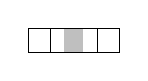
\begin{tikzpicture}
			\tikztapeax
		\end{tikzpicture}%
}}

%%% ALL THE DRAWINGS ARE UPDATED TO THE xa^Ky FORM
\newcommand{\leftloop}{\raiseTikz{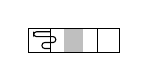
\begin{tikzpicture}
			\tikztapeax
			\draw [rounded corners=1pt] (8pt,1.7ex) -- (2pt,1.7ex) -- (2pt,1.3ex) -- (10pt,1.3ex) -- (10pt,.8ex) -- (5pt,.8ex) -- (5pt,0.3ex) -- (8pt,0.3ex);
		\end{tikzpicture}%
}}

\newcommand{\rightloop}{\raiseTikz{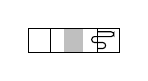
\begin{tikzpicture}
			\tikztapeax
			\draw [rounded corners=1pt] (25pt,1.7ex) -- (31pt,1.7ex) -- (31pt,1.3ex) -- (23pt,1.3ex) -- (23pt,.8ex) -- (28pt,.8ex) -- (28pt,0.3ex) -- (25pt,0.3ex);
		\end{tikzpicture}%
}}

\newcommand{\leftsink}{\raiseTikz{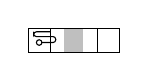
\begin{tikzpicture}
			\tikztapeax
			\draw [rounded corners=1pt] (8pt,1.7ex) -- (2pt,1.7ex) -- (2pt,1.3ex) -- (10pt,1.3ex) -- (10pt,.8ex) -- (5pt,.8ex);
			\draw (4pt,0.8ex) circle (1pt);
		\end{tikzpicture}%
}}

\newcommand{\rightsink}{\raiseTikz{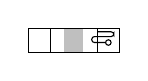
\begin{tikzpicture}
			\tikztapeax
			\draw [rounded corners=1pt] (25pt,1.7ex) -- (31pt,1.7ex) -- (31pt,1.3ex) -- (23pt,1.3ex) -- (23pt,.8ex) -- (28pt,.8ex);
			\draw (29pt,0.8ex) circle (1pt);
		\end{tikzpicture}%
}}

\newcommand{\rightcrossing}{\raiseTikz{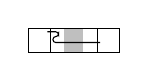
\begin{tikzpicture}
			\tikztapeax
			\draw [rounded corners=1pt] (7pt,1.7ex) -- (11pt,1.7ex) -- (11pt,1.3ex) -- (9pt,1.3ex) -- (9pt,.8ex) -- (26pt,.8ex);
		\end{tikzpicture}%
}}

\newcommand{\leftcrossing}{\raiseTikz{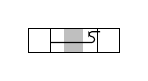
\begin{tikzpicture}
			\tikztapeax
			\draw [rounded corners=1pt] (26pt,1.7ex) -- (22pt,1.7ex) -- (22pt,1.3ex) -- (24pt,1.3ex) -- (24pt,.8ex) -- (8pt,.8ex);
		\end{tikzpicture}%
}}


\newcommand{\mysubparagraph}[1]{\noindent \textbf{\textsf{#1}} }
%\newcommand{\mysubpar}[1]{{\noindent \textsf{\textbf{#1}}}}

\begin{document}
	
	\maketitle
	
	\begin{abstract}
		One Counter Nets (OCNs) are finite-state automata equipped with a counter that
		cannot become negative, but cannot be explicitly tested for zero. Their close
		connection to various other models (e.g., PDAs, Vector Addition Systems, and
		Counter Automata) make them an attractive modeling tool.
		
		The two-way variant of OCNs (2-OCNs) was introduced in the 1980's and shown to
		be more expressive than OCNs, so much so that the emptiness problem is
		undecidable already in the deterministic model (2-DOCNs).
		
		In a first part, we study the emptiness problem of natural restrictions of
		2-OCNs, under the light of modern results about Vector Addition System with
		States (VASS).  We show that emptiness is decidable for 2-OCNs over
		\emph{bounded languages} (i.e., languages contained in
		$a_1^*a_2^*\cdots a_k^*$), and decidable and Ackermann-complete for \emph{sweeping}
		2-OCNs, where the head direction only changes at the end-markers. Both
		decidability results revolve around reducing the problem to VASS reachability,
		but they rely on strikingly different approaches.  In a second part, we study
		the expressive power of 2-OCNs, showing an array of connections between
		bounded languages, sweeping 2-OCNs, and semilinear languages.  Most noteworthy
		among these connections, is that the bounded languages recognized by sweeping
		2-OCNs are precisely those that are semilinear. Finally, we establish an
		intricate pumping lemma for 2-DOCNs and use it to show that there are OCN
		languages that are not 2-DOCN recognizable, improving on the known result that
		there are such 2-OCN languages.
		
		%%%%
		% We study the two-way variant of OCNs (2-OCNs) that can move their read-only
		% head back and forth on the input tape. We show that this variant is far more
		% expressive than OCNs, so much so that the emptiness problem is undecidable
		% already in the deterministic model (2-DOCNs).  We proceed to study the
		% emptiness problem for natural restrictions of 2-OCNs, showing that it is
		% decidable for 2-OCNs over \emph{bounded languages} (i.e., languages contained
		% in $a_1^*a_2^*\cdots a_k^*$), and decidable and Ackermann-complete for
		% \emph{sweeping} 2-OCNs, where the head direction only changes at the end-markers.  Both decidability results revolve around reducing the problem to
		% VASS reachability, but they rely on strikingly different approaches.  We also
		% study the expressive power of 2-OCNs, showing an array of connections between
		% bounded languages, sweeping 2-OCNs, and semilinear languages.  Most noteworthy
		% among these connections, is that the bounded languages recognized by sweeping
		% 2-OCNs are precisely those that are semilinear.  Finally, we show that 2-OCNs
		% are more expressive than 2-DOCN, by establishing an intricate pumping lemma
		% for 2-DOCNs.
	\end{abstract}
	\section{Introduction}
	A \emph{One-Counter Net (OCN)} is a finite state automaton equipped with a
	counter that cannot decrease below zero, but cannot be explicitly tested for
	zero.  It is a natural restriction of several computational models: One-Counter
	Automata without zero tests, and Pushdown
	Automata with a single letter stack alphabet. It can also be thought of as
	1-dimensional Vector Addition Systems with accepting States and an alphabet.
	
	OCNs are an attractive model for studying the border of decidability, as several
	problems for them lie close to the decidability frontier (e.g., both
	determinization and universality may be decidable or undecidable, depending on
	the precise definition and context
	\cite{hofman2013decidability,hofman2014trace,almagor2020parametrized,almagor2022determinization,almagor2024dimension}).
	%add~\cite{almagor2024} after publication
	
	OCNs suffer from an unsettling asymmetry: the language
	$L=\left\{a^nb^m \mid n \geq m\right\}$ is OCN-recognizable (by counting $+1$ on
	$a$ and $-1$ on $b$), whereas the language $\left\{a^nb^m \mid n \leq m\right\}$ is
	not OCN-recognizable. In particular, they are not closed under reversal (nor
	under intersection).  A natural way of making OCNs more robust is therefore to
	look at their two-way variant. 
	
	This approach was taken in~\cite{miyano1982two,chan1987two}, where the model of \emph{two-way one-counter nets (2-OCNs)} is introduced and studies. A 2-OCN is a one counter net that receives its input on a tape, surrounded by end-markers $\lmark$ and $\rmark$, and is allowed to move a read-only head back and forth on the tape.
	As the following examples witness, the introduction of a two-way tape
	significantly increases the expressive power of the model, as well as its
	deterministic fragment \emph{(2-DOCN)}. For uniformity, we henceforth refer to one-way OCNs as \emph{1-OCN}.
	\begin{example}
		\label{xmp:aNbN} Consider the language $L_1=\{a^nb^n\mid n\in \bbN\}$, which is
		easily shown not to be 1-OCN-recognizable.  $L_1$ can be recognized by a 2-OCN
		(in fact 2-DOCN, see Fig.~\ref{fig:aNbN_reset}) by using a ``counter reset'':
		it starts with a forward scan verifying that the format is $a^nb^m$ while
		counting $+1$ on $a$ and $-1$ on $b$. Thus, upon reaching $\rmark$, the
		counter has value $n-m$ (unless $n<m$, in which case the run terminates due to
		the counter becoming negative, and the word is not accepted), and in
		particular $n\ge m$.  It then moves backwards to $\lmark$, counting $-1$ on
		$a$ and $+1$ on $b$, thus resetting the counter back to $0$. Next, it goes
		forward again to $\rmark$, then similarly computes $m-n$ from right to
		left. Intuitively, this approach recognizes
		$\{a^nb^m\mid n\ge m\}\cap \{a^nb^m\mid n\le m\}$ and uses the closure of 2-DOCN under intersection~\cite{miyano1982two}.
		\begin{figure}[ht]
			\begin{minipage}{.72\textwidth}
				\footnotesize 
				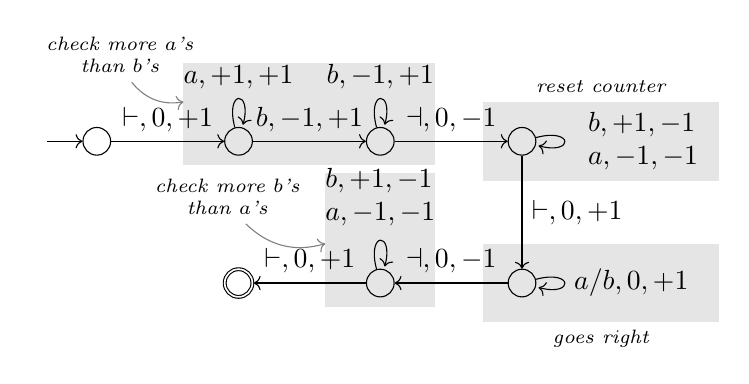
\begin{tikzpicture}[->,node distance=1.8cm, every
					state/.style={minimum size=10pt, inner sep=2pt}]
					\node[state, initial text=,initial left](A){};
					\node[state, right of=A](B){};
					\node[state, right of=B](C){};
					\node[state, right of=C](D){};
					\node[state, below of=D](E){};
					\node[state, left of=E](F){};
					\node[state, left of=F, accepting](G){};
					\draw (A) edge[above] node{$\trans{\lmark}{0}{+1}$} (B) (B) edge[loop
					above] node{$\trans{a}{+1}{+1}$} (B) (B) edge[above]
					node{$\trans{b}{-1}{+1}$} (C) (C) edge[loop above]
					node{$\trans{b}{-1}{+1}$} (B) (C) edge[above]
					node{$\trans{\rmark}{0}{-1}$} (D) (D) edge[loop right] node {%
						$
						\begin{array}{l}
							\trans{b}{+1}{-1}\\
							\trans{a}{-1}{-1}
						\end{array} $} (D)
					(D) edge[right] node{$\trans{\lmark}{0}{+1}$} (E) (E) edge[loop right]
					node{$\trans{a/b}{0}{+1}$} (E) (E) edge[above]
					node{$\trans{\rmark}{0}{-1}$} (F) (F) edge[loop above] node{%
						$
						\begin{array}{l}
							\trans{b}{+1}{-1}\\
							\trans{a}{-1}{-1}
						\end{array}$} (F) (F) edge[above] node{$\trans{\lmark}{0}{+1}$} (G);
					\begin{scope}[on background layer,every node/.style={font=\it\scriptsize}]
						\fill[black!10] ($(B)+(-.7cm, -.3cm)$) rectangle ($(C)+(.7cm, 1cm)$);
						\node[anchor=east,align=center] (b) at ($(B)+(-.45cm, 1.1cm)$) {check
							more \(a\)'s\\ than \(b\)'s};
						\draw[black!50,bend right,->] (b) edge ($(B)+(-.7cm,.5cm)$);
						\fill[black!10] ($(D)+(-.5cm, -.5cm)$) rectangle ($(D)+(2.5cm,
						.5cm)$);
						\node at ($(D)+(1cm, .7cm)$) {reset counter};
						\fill[black!10] ($(E)+(-.5cm, -.5cm)$) rectangle ($(E)+(2.5cm,
						.5cm)$);
						\node at ($(E)+(1cm, -.7cm)$) {goes right};
						\fill[black!10] ($(F)+(-.7cm, -.3cm)$) rectangle ($(F)+(.7cm, 1.4cm)$);
						\node[anchor=east,align=center] (b) at ($(F)+(-.9cm, 1.1cm)$) {check
							more \(b\)'s\\ than \(a\)'s};
						\draw[black!50,bend right,->] (b) edge ($(F)+(-.7cm,.5cm)$);
					\end{scope}
				\end{tikzpicture}
				\caption{2-DOCN recognizing $\{a^nb^n\mid n\in \bbN\}$ using counter-reset. A transition $\sigma,e,h$ means ``read letter $\sigma$, change counter by $e$, and move head by $h$''.}
				\label{fig:aNbN_reset}
			\end{minipage}
			\quad%
			\begin{minipage}{.24\textwidth}
				\footnotesize
				\newcommand{\blk}[2]{\subnode{#1}{#2}}
				\begin{tikzpicture}[remember picture]
					\node (w) at (0,1.8) {$\lmark \blk{n1}{aaa}\#\blk{n2}{aa}\#\blk{n3}{aaa}\#\blk{n4}{a}\#\rmark$};
					\draw [-{Latex[length=4pt]}] (-1.5,1.2) -- (-0.7,1.2) node[midway,above=-2pt]{+3};
					\draw [-{Latex[length=4pt]},dashed] (-0.7,1.2) -- (-0.1,1.2) node[midway,above=-2pt]{0};
					\draw [-{Latex[length=4pt]}] (-0.1,1.2) -- (0.6,1.2) node[midway,above=-2pt]{-3};
					\draw [-{Latex[length=4pt]},rounded corners=4pt] (0.5,1.2) -- (0.7,1.2) -- (0.7,0.8) -- (0.4,0.8);
					\draw [-{Latex[length=4pt]}] (0.6,0.8) -- (-0.2,0.8) node[midway,above=-2pt]{+6};
					\draw [-{Latex[length=4pt]}] (-0.2,0.8) -- (-1.3,0.8) node[midway,above=-2pt]{0};
					\draw [-{Latex[length=4pt]},rounded corners=4pt] (-1.3,0.8) -- (-1.5,0.8) -- (-1.5,0.4) -- (-1.2,0.4);
					\draw [-{Latex[length=4pt]}] (-1.4,0.4) -- (-0.7,0.4) node[midway,above=-2pt]{-6};
					\node (acc) at (-0.2,0.5) {accept};
					\useasboundingbox (current bounding box.north east) rectangle (current
					bounding box.south west);
					\foreach \i in {1, ..., 4} {
						\path let \p1 = ($(w) + (0, 0.3cm)$)
						in node[font=\tiny] at (\p1 -| n\i) {\(a^{n_\i}\)};
					}
					\begin{scope}[on background layer]
						\foreach \i in {1, 3} {
							\fill[black!10] (n\i.south west) rectangle (n\i.north east);
						}
					\end{scope}
				\end{tikzpicture}
				\caption{An accepting run of a 2-OCN for $L_2$. The dashed line signifies a nondeterministic guess. }
				\label{fig:example_2_2}
			\end{minipage}
		\end{figure}
	\end{example}
	The next example demonstrates the fact~\cite{chan1987two} that 2-OCN are more expressive than 2-DOCN. In addition, it demonstrates that sometimes it is (seemingly) necessary for the head to ``change direction'' inside the tape, rather than at the end markers. 
	\begin{example}
		\label{xmp:nondet_aNbN} Let \(L_2\) be the language
		$\{a^{n_1}\#\cdots \#a^{n_k}\#\mid k\in \bbN\wedge (\exists i > 1)[n_1=n_i]\}$, i.e., words where the length of the first $a$-segment is matched in some later segment. This language
		is not 1-OCN recognizable, and one may observe that a similar approach
		to~\cref{xmp:aNbN} fails, because we would need to guess the index $i$ for
		which $n_1=n_i$, but in order to reset the counter, we must ``forget'' the
		guess. Thus, in order to recognize this with a 2-OCN, we must compare $n_1$
		to $n_i$ via a single visit to the $i$-th segment.
		
		To achieve this, the 2-OCN counts $+1$ on
		the first segment $a^{n_1}$, then scans forward and guesses when the
		correct segment $i$ is reached. It then counts $-1$ on $a^{n_i}$. Thus,
		upon reaching $\#$, the counter holds $n_1-n_i$ (and so guarantees that
		$n_1\ge n_i$ if it survives).  Then, a backward scan is performed from $\#$
		counting $+2$ on $a$ in $a^{n_i}$, until $\#$ is reached, and then
		continues left to $\lmark$ and finally counts $-2$ on the $a$'s in
		$a^{n_1}$.  Thus, the counter ends with value
		$n_1-n_i+2n_i-2n_1=n_i-n_1$. Again, if $n_i<n_1$ the run terminates, so the
		whole run survives if $n_1\le n_i$, which combined with $n_1\ge n_i$ gives $n_1=n_i$ (see Fig.~\ref{fig:example_2_2}).
	\end{example}
	A 2-OCN that only changes its head direction at the end marks is called
	\emph{sweeping}. \Cref{xmp:nondet_aNbN} prompts studying the expressive power of
	sweeping 2-OCNs, which we take on in this work.
	
	\subparagraph*{Related Work.} Two-way automata have received much attention since
	their introduction for finite automata in~\cite{rabin1959finite}. 2-PDAs were
	studied
	in~\cite{martin1973two,gray1967two,arikawa1968some,monien1984deterministic},
	focusing mainly on closure properties and languages recognizable by 2-PDAs.  It
	is claimed in~\cite{arikawa1968some} that~\cite{gray1967two} exhibit a language
	not in 2-PDA, but this seems to be an error, as no such language is described.
	No techniques are known to the authors to show that some languages is not
	expressible with a 2-PDA, and most questions about 2-PDA, including whether the
	deterministic variant can recognize all context-free languages, are
	open~\cite{galil1976some}.
	
	In the world of counter machines,~\cite{duris1982fooling} shows that DFAs with a
	``blind tape'' (a form of a nonnegative counter that cannot be 0-tested) are
	less expressive than 2-DPDAs.  A significant body of work by Ibarra et
	al. studies \emph{reversal bounded}
	counters~\cite{ibarra1993equivalence,ibarra1999counter,ibarra2004two,dang2005two,ibarra1995new},
	i.e., counters that cannot increase and decrease unboundedly many times. The heavy reliance
	on reversal-boundedness makes these works orthogonal to ours. Atig and Ganty~\cite{atig2011approximating} study a VASS-CFG hybrid, and use also make use of reductions to VASS with 0-tests, but with significant technical differences.
	
	Closer to our setting are \emph{two-way one-counter automata} (2-OCAs), that
	allow explicit zero tests. In~\cite{petersen1994two} certain languages computing
	squaring or exponentiation are shown not to be 2-DOCA recognizable (the
	deterministic variant), whereas~\cite{de2014unary} exhibit nonsemilinear 2-OCA
	languages.  Ibarra and Su~\cite{ibarra1999counter} note that 1-sweep 2-DOCA have
	an undecidable emptiness problem; in contrast, we show that this problem is
	decidable for sweeping 2-OCN.  They also note that, over bounded languages,
	emptiness of 2-DOCA is decidable \emph{provided} that the counter reaches zero
	only a constant number of times; in contrast, we show that this emptiness over
	bounded languages is decidable for any 2-OCN. 
	
	A nearly identical model to 2-OCN has been introduced in~\cite{miyano1982two} and further studied in~\cite{chan1987two}. In their model, the counter updates are $\pm 1$, which essentially amounts to encoding counters in unary.
	In~\cite{miyano1982two}, the focus is on 2-DOCN recognizable languages. It is shown that this class is closed under intersection, but not under complementation nor union. Further, over bounded languages, 2-DOCN can be made sweeping\footnote{The proof in~\cite{miyano1982two} is actually missing significant details, but those can be reconstructed.}, and the Parikh images of their languages are semilinear. 
	An example is also given to show that 2-DOCN are less expressive than 2-OCN.
	
	The algorithmic contribution in~\cite{chan1987two} is that the emptiness problem for 2-DOCN is undecidable. Additionally, it is shown that if a 2-OCN accepts a word of length $n$, then it accepts it with a run of polynomial length in $n$. The latter result no longer holds for our model, due to the binary encoding of the counters.
	
	
	\subparagraph*{Contribution and Paper Organization.}  In this work we
	provide a modern view of 2-OCNs and some of its interesting and decidable
	fragments, namely \emph{bounded-language 2-OCNs} and \emph{sweeping
		2-OCNs}. In~\cref{sec:DOCN_undec} we give a counter-machine based proof of the
	undecidability of 2-DOCN emptiness.  In~\cref{sec:bounded_languages}, we
	consider 2-OCNs whose languages are \emph{bounded}, i.e., of the form
	$L\subseteq a_1^*a_2^*\cdots a_k^*$.  We show that under this restriction, emptiness becomes
	decidable. In~\cref{sec:sweeping}, we consider \emph{sweeping} 2-OCNs, i.e.,
	2-OCNs whose head-movement direction only changes at the end-markers.  We show
	that here too emptiness becomes decidable and we give precise complexity bounds,
	using recent results regarding VASS reachability.  In~\cref{sec:semilinear}, we
	investigate the relationship between semilinear languages and 2-OCN
	languages. We show that for bounded languages, the set of \emph{lengths} of
	words in the language of a 2-OCN is semilinear, and derive explicit languages
	that are not 2-OCN-recognizable.  We also show that a bounded language is
	semilinear if and only if it is recognizable by a sweeping 2-OCN.
	In~\cref{sec:nondet_vs_det}, we show an elaborate pumping lemma for
	2-DOCNs. Apart from its independent usefulness for understanding 2-DOCNs, this
	enables us to demonstrate a 1-OCN whose language is not 2-DOCN recognizable,
	establishing a new separation result.  We conclude
	in~\cref{sec:results_directions} with some open problems.
	
	% Our focus in this work is on 
	% the emptiness problem for 2-OCNs and 2-DOCNs, and their expressive power.
	% In~\cref{sec:prelim}, we introduce the model of
	% 2-OCNs. In~\cref{sec:DOCN_undec}, we show that the emptiness problem is
	% undecidable already for 2-DOCNs. We then turn our focus to two interesting
	% fragments of 2-OCNs, namely \emph{bounded-language 2-OCNs} and \emph{sweeping
		%   2-OCNs}.  In~\cref{sec:bounded_languages}, we consider 2-OCNs whose languages
	% are \emph{bounded}, i.e., of the form $L\subseteq a_1^*a_2^*\cdots a_k^*$. We show that under
	% this restriction, emptiness becomes decidable. In~\cref{sec:sweeping}, we
	% consider \emph{sweeping} 2-OCNs, i.e., 2-OCNs whose head-movement direction only
	% changes at the end-markers. We show that here too emptiness becomes decidable
	% and we give precise complexity bounds.  In~\cref{sec:semilinear}, we investigate
	% the relationship between semilinear languages and 2-OCN languages. We show that
	% for bounded languages, the set of \emph{lengths} of words in the language of a
	% 2-OCN is semilinear, and derive explicit languages that are not
	% 2-OCN-recognizable.  We also show that a bounded language is semilinear if and
	% only if it is recognizable by a sweeping 2-OCN.  In~\cref{sec:nondet_vs_det}, we
	% show that 2-OCNs are strictly more expressive than 2-DOCNs.  To this end, we
	% show an elaborate pumping lemma for 2-DOCNs. We conclude
	% in~\cref{sec:results_directions} with some additional results and open problems.
	
	We encourage the reader to initially skip the proofs and garner a bird's eye view of our results. 
	%\shtodo{rephrase this to encourage reading appendix proofs?}
	%We encourage the reader, upon first reading, to skip the proofs altogether in
	%order to garner a bird's eye view of our results.  
	Thereafter, we note that
	\cref{sec:2OCN_Bounded_to_VASS_intuitive,lem:correctness_Bounded_2OCN_to_VASS,thm:bounded_sweeping_equiv_semilinear,lem:2DOCN_pump}
	have the most interesting proofs. Detailed proofs appear in the appendix.
	
	
	
	
	
	\section{Preliminaries}
	\label{sec:prelim}
	\subparagraph*{Two-Way OCN and Automata.} For an alphabet set $\Sigma$, we denote
	$\Sigma_{\lmark\rmark}=\Sigma\cup \{\lmark,\rmark\}$ where $\lmark,\rmark$ are two symbols
	not appearing in $\Sigma$, called \emph{left end-marker} and \emph{right end-marker},
	respectively.  A \emph{Two-Way One-Counter Net (2-OCN)} is a tuple
	$\cA=\tup{Q,\Sigma,\Delta,\initstate,\accstate}$ where $Q$ is a finite set
	of \emph{states}, $\Sigma$ is a finite alphabet, $\Delta\subseteq
	Q\times \Sigma_{\lmark\rmark}\times \bbZ\times \{-1,+1\}\times Q$ is a finite set of \emph{transitions}, $\initstate,\accstate\in Q$ are the initial and accepting states, respectively. 
	Intuitively, a transition $\tau=(q,\sigma,e,h,q')$ dictates that from state $q$, when reading letter $\sigma$, we add $e$ to the counter value, move the position of the head on the tape by $h$, and reach state $q'$. We call $e$ 
	the \emph{effect} and  $h$ the \emph{head shift} of the transition. Unless explicitly stated otherwise, we assume that the effect $e$ is encoded in binary.
	We require that if $(q,\lmark,e,h,q')\in \Delta$ then $h=1$ and if
	$(q,\rmark,e,h,q')\in \Delta$ then $h=-1$. That is, upon reaching the end-markers, the head cannot proceed beyond them.
	
	We say that $\cA$ is \emph{deterministic} (denoted 2-DOCN) if for every $q\in
	Q,\sigma\in \Sigma_{\lmark,\rmark}$ there is at most one $q'\in Q$ and $e,h$ such that
	$(q,\sigma,e,h,q')$. We say that $\cA$ is \emph{one way} (denoted 1-OCN) if every
	transition moves the head to the right (i.e., the head shift is 1).
	
	A \emph{configuration} of $\cA$ is $(q,c,p)\in Q\times \bbN\times \bbN$ representing the
	current state $q$, counter value $c$, and head position $p$. Note that we do not
	consider configurations with negative counter values, thus enforcing the
	semantics of Counter Nets.
	% 
	Consider a word $w=\sigma_1\cdots \sigma_m\in \Sigma^*$, we augment it to $\lmark w\rmark$ by setting
	$\sigma_0=\,\lmark$ and $\sigma_{m+1}=\,\rmark$.  A \emph{run} of $\cA$ on $w$ is a finite
	sequence of configurations $\rho=(q_1,c_1,p_1),(q_2,c_2,p_2),\ldots,(q_{n},c_{n},p_{n})$
	such that $0\le p_i\le m+1$ for all \(i\), and for every $1\le i< n$ we have
	$(q_{i},\sigma_{p_i},c_{i+1}-c_i,p_{i+1}-p_i,q_{i+1})\in \Delta$. That is, each
	configuration follows from the previous one by the transition relation.  A run
	is \emph{initial} if $q_1=\initstate$ and $p_1=c_1=0$. A run is \emph{accepting}
	if $q_n=\accstate$. We tacitly assume that runs do not continue after the
	accepting state. The word $w$ is accepted by $\cA$ if $\cA$ has an initial and accepting
	run on it. We define $L(\cA)=\{w\in \Sigma^* \mid \cA \text{ accepts }w\}$. Note that, just like OCNs, 2-OCNs are \emph{monotone}, i.e., every word accepted from initial configuration $(q,c,p)$ is also accepted from $(q,c',p)$ for every $c'>c$. We sometimes
	consider sequences of pseudo-configurations where the counter value becomes
	negative. In such cases, we say that the run is \emph{cut short by a counter
		violation}, and we mean that the sequence of configurations is a run up to a
	prefix in which the counter becomes negative.
	
	Finally, we sometimes discuss classical Boolean automata (NFA, DFA, 2-NFA and
	2-DFA). For our purposes, they can be thought of as 2-OCN where all the counter
	updates are $0$, and are therefore omitted.
	
	
	\subparagraph*{VASS and VASS with bounded 0-tests.} A \emph{Vector Addition
		System with States (VASS)} is a tuple $\cV=\tup{S,T}$ where $S$ is a finite
	set of states and $T\subseteq S\times \bbZ^d\times S$ is the transition relation. A
	\emph{configuration} of $T$ is $(s,\vec{v})$ where $s\in S$ and
	$\vec{v}\in \bbN^d$ (note that this is a vector of nonnegative integers). We say
	that configuration $(s_2,\vec{y})$ is \emph{reachable} from configuration
	$(s_1,\vec{x})$ if there is a finite sequence of configurations
	$(p_1,\vec{v_1}),\ldots,(p_m,\vec{v_m})$ such that
	$(p_1,\vec{v_1})=(s_2,\vec{y}), (p_m,\vec{v_m})=(s_2,\vec{y})$ and for every
	$1\le i<m$ we have $(p_i,\vec{v_{i+1}}-\vec{v_i},p_{i+1})\in T$.  Intuitively, a
	VASS runs by repeatedly adding vectors to the configuration, as long as all the
	\emph{counters} (i.e., the entries of the vector) remain nonnegative.  The
	reachability problem for VASS asks whether $(s_2,\vec{y})$ is reachable from
	$(s_1,\vec{x})$ and is known to be decidable~\cite{czerwinski2022reachability}.
	
	While VASS do not allow explicit 0-tests, it is possible to simulate a fixed
	number of 0-tests within the context of
	reachability~\cite{czerwinski2020reachability,czerwinski2022reachability}. That
	is, we can extend the transition relation so that $T\subseteq S\times \bbZ^d\times \{=0,\ge 0\}^d \times
	S$, and a transition can be taken only when the counters that have $=0$ tests
	are 0. As long as there is a constant \(B\) such that there are no more than $B$
	0-tests along every run of the VASS, then reachability remains decidable.  The
	simplest approach to achieve this is to increase the dimension by $d\cdot B$,
	keeping $B$ copies of every counter, and whenever a counter needs to be tested
	for 0, a copy of it is ``frozen'' (i.e., never changes again) and the
	reachability target has $0$ on all frozen entries. Note that we can mark which
	entries are frozen in the states of the VASS, since there are at most $B$ of
	them. We remark that more elaborate approaches can keep the number of added
	counters small~\cite{czerwinski2020reachability,czerwinski2022reachability}.  We
	call such machines \emph{VASS with bounded 0-tests}.
	
	\section{The Emptiness and Membership Problems in 2-OCNs and Variants}
	\subsection{Emptiness of 2-DOCNs is Undecidable}
	\label{sec:DOCN_undec}
	%We show that 
	It is shown in~\cite{chan1987two} that already for 2-DOCNs, the emptiness problem, namely the problem of deciding whether $L(\cD)= \emptyset$ for a given 2-DOCN $\cD$, is undecidable. This is shown by a reduction from Hilbert's 10th problem. More precisely, it is shown that 2-DOCN can simulate multiplication, in a sense.
	
	An arguably cleaner way of obtaining this result while staying in the world of
	counter machines, is via reduction from the halting problem for Two-Counter
	Machines, as follows:
	%One way to obtain this result is to extend~\cref{xmp:multiplication} to capture Diophantine equations using 2-DOCN. While this is fairly straightforward, in Appendix~\ref{apx:2DOC_emptiness_undecidable} we opt to
	%use a cleaner reduction that stays in the world of counter machines, and conclude the following.
	
	% \subparagraph*{Two-Counter Machines.}  A \emph{two-counter machine}~\cite{minsky1967computation}
	% (or Minsky Machine) $\cM$ is a sequence $(l_1,\ldots,l_n)$ of commands involving two
	% counters $x$ and $y$. We refer to $\{1,\ldots,n\}$ as the {\em locations} of the
	% machine. There are five possible forms of commands:
	% \texttt{inc(c)}, \texttt{dec(c)}, \texttt{goto $l_i$}, \texttt{halt}, \texttt{if
		%   c=0 goto $l_i$ else goto $l_j$}, where $\texttt{c}\in \{x,y\}$ is a counter and $1\le i,j\le n$
	% are locations.  The counters are initially set to $0$.  Since we can always
	% check whether $\texttt{c}=0$ before a $\texttt{dec(c)}$ command, we assume that the
	% machine never reaches $\texttt{dec(c)}$ with $\texttt{c}=0$. That is, the counters never
	% have negative values.
	\begin{theorem}[\cite{chan1987two}]
		\label{thm:2DOCN_emptinesss_undecidable} The emptiness problem for 2-DOCN
		is undecidable.
	\end{theorem}
	%\begin{proof}[Proof Sketch (see Appendix~\ref{apx:2DOC_emptiness_undecidable})]
	%   We show the undecidability of 2-DOCN emptiness by reduction from the
	%   (complement of the) halting problem for two-counter machines, which is known to be
	%   undecidable~\cite{minsky1967computation}.
	
	%   Given a two-counter machine $\cM$, we construct a 2-DOCA $\cA$ which reads
	%   input words of the form $\#(x^*y^*\#)^*$, representing the values of the
	%   counters $x$ and $y$ along the run of $\cM$, with each step of the machine
	%   separated with $\#$.  Intuitively, $\cA$ tracks the location of $\cM$ in its
	%   state, uses the counter values to determine the location after a jump, and at
	%   each steps checks that the counter values between steps are consistent,
	%   similarly to \cref{xmp:aNbN}. Then, $\cA$ accepts if at any point the
	%   computation reaches the location $\texttt{halt}$. If a counter violation is
	%   encountered, $\cA$ moves to a rejecting sink.
	%%%%%%%%%%%%%%%%%%%%%%%%
	% More precisely, $\cA$ starts by checking (using a single right-to-left pass
	% with a DFA) that the word adheres to the format $\#(x^*y^*\#)^*$. It then
	% resets the head to $\lmark$, records the location $l_1$ in its state, moves
	% the head to the first $\#$ and begins the simulation.  $\cA$ simulates each
	% step starting from the $\#$ preceding the segment $x^my^k$ representing the
	% current counter values, and along the simulation scans only the segment of the
	% word of the form $\#x^my^k\#x^{m'}y^{m'}\#$ starting at the current head
	% location.  Note that crucially, the format of the segment is fixed, so that
	% the head can end the simulation in the middle $\#$, thus correctly viewing the
	% counter values of the next step.
	%
	% If the command at the current location is \texttt{goto $l_i$}, then $\cA$
	% checks that $m=m'$ and $k=k'$, similarly to \cref{xmp:aNbN}. Similarly, if the
	% current command is e.g., $\texttt{inc(x)}$ or $\texttt{dec(y)}$, then $\cA$
	% checks that $k'=k+1$ and $m=m'$, or that $k=k'$ and $m'=m-1$, respectively, by
	% a similar comparison prefixed by a $\pm1$ counter change.
	%
	% If the current command is e.g., \texttt{if x=0 goto $l_i$ else goto $l_j$},
	% then $\cA$ checks that $k=k'$ and $m=m'$, and then checks whether $k=0$ (by
	% checking if there are any $x$'s after the first $\#$ in the segment), and if
	% so moves to $l_i$ and otherwise to $l_j$.
	%
	% Finally, if $\cA$ ever reaches the command $\texttt{halt}$, it accepts, and if
	% any of the comparisons fails, the counter goes below 0 and the word is
	% rejected. If $\rmark$ is reached without reaching $\texttt{halt}$, then $\cA$
	% moves to a rejecting sink.
	%
	% We then have that $L(\cA)\neq \emptyset$ if and only if there exists a word representing
	% the counter values in a halting run of $\cM$, if and only if $\cM$ halts.
	% \end{proof}
\begin{proof}
	We show the undecidability of 2-DOCN emptiness by reduction from the
	(complement of the) halting problem for two-counter machines, which is known to be
	undecidable~\cite{minsky1967computation}.
	
	Given a two-counter machine $\cM$, we construct a 2-DOCA $\cA$ which reads
	input words of the form $\#(x^*y^*\#)^*$, representing the values of the
	counters $x$ and $y$ along the run of $\cM$, with each step of the machine
	separated with $\#$.  Intuitively, $\cA$ tracks the location of $\cM$ in its
	state, uses the counter values to determine the location after a jump, and at
	each steps checks that the counter values between steps are consistent,
	similarly to \cref{xmp:aNbN}.  Then, $\cA$ accepts if at any point the
	computation reaches the location $\texttt{halt}$. If a counter violation is
	encountered, $\cA$ moves to a rejecting sink.
	
	More precisely, $\cA$ starts by checking (using a single right-to-left pass
	with a DFA) that the word adheres to the format $\#(x^*y^*\#)^*$. It then
	resets the head to $\lmark$, records the location $l_1$ in its state, moves
	the head to the first $\#$ and begins the simulation.  $\cA$ simulates each
	step starting from the $\#$ preceding the segment $x^my^k$ representing the
	current counter values, and along the simulation scans only the segment of the
	word of the form $\#x^my^k\#x^{m'}y^{m'}\#$ starting at the current head
	location.  Note that crucially, the format of the segment is fixed, so that
	the head can end the simulation in the middle $\#$, thus correctly viewing the
	counter values of the next step.
	
	If the command at the current location is \texttt{goto $l_i$}, then $\cA$
	checks that $m=m'$ and $k=k'$, similarly to \cref{xmp:aNbN}. Similarly, if the
	current command is $\texttt{inc(x)}$ or $\texttt{dec(y)}$, then $\cA$
	checks that $k'=k+1$ and $m=m'$, or that $k=k'$ and $m'=m-1$, respectively, by
	a similar comparison prefixed by a $\pm1$ counter change.
	
	If the current command is \texttt{if x=0 goto $l_i$ else goto $l_j$},
	then $\cA$ checks that $k=k'$ and $m=m'$, and then checks whether $k=0$ (by
	checking if there are any $x$'s after the first $\#$ in the segment), and if
	so moves to $l_i$ and otherwise to $l_j$.
	
	Finally, if $\cA$ ever reaches the command $\texttt{halt}$, it accepts, and if
	any of the comparisons fails, the counter goes below 0 and the word is
	rejected. If $\rmark$ is reached without reaching $\texttt{halt}$, then $\cA$
	moves to a rejecting sink.
	
	We then have that $L(\cA)\neq \emptyset$ if and only if there exists a word representing
	the counter values in a halting run of $\cM$, if and only if $\cM$ halts.
\end{proof}


\subsection{Emptiness of 2-OCNs over Bounded Languages is Decidable}
\label{sec:bounded_languages}
\label{sec:2OCN_Bounded_to_VASS_intuitive} 
Consider an alphabet $\Sigma=\{a_1,\ldots,a_k\}$. A language $L$ is \emph{bounded} if $L\subseteq
a_1^*a_2^*\cdots a_k^*$. In this section, we show that the emptiness problem of
2-OCNs over bounded languages is decidable.
\begin{remark} %[General Bounded Languages]
	Generally, a bounded language is a subset of $x_1^*x_2^*\cdots x_k^*$ where each
	$x_i\in \Sigma^*$ (in particular, e.g., $a^*b^*a^*$ is also bounded). Our results
	readily extend to these languages, but they add a cumbersome notational
	layer, which we opt to avoid.
\end{remark}
%\shtodo{Probably shorten below}
\begin{theorem}
	\label{thm:emptiness_bounded_decidable} The following problem is decidable:
	given a 2-OCN $\cA$ is $L(\cA)\cap a_1^*a_2^*\cdots a_k^* = \emptyset$?
\end{theorem} 
We prove \cref{thm:emptiness_bounded_decidable} in the remainder of this section. The proof is by reduction to the VASS nonreachability problem, known to be
Ackermann-complete~\cite{czerwinski2022reachability}. 

%\subsection{From 2-OCN with Bounded Language to VASS}
Consider a 2-OCN $\cA$. We henceforth assume that membership in $a_1^*a_2^*\cdots a_k^*$ is already
tested within $\cA$, i.e., that $L(\cA)$ is a bounded language. We further assume
that $L(\cA)\subseteq a_1^+a_2^+\cdots a_k^+$, namely that every letter occurs at least once
in every word in $L$ (dubbed \emph{properly-bounded}). Indeed, for the purpose
of emptiness we can split $L(\cA)$ to a union over all subsets $\Gamma\subseteq \Sigma$ of
properly-bounded languages over $\Gamma$.

We obtain from $\cA$ a VASS with bounded 0-tests $\cV$ such that $L(\cA)\neq \emptyset$ iff
$(s_{\textrm{init}},\vec{0})$ reaches $(s_{\textrm{fin}},\vec{0})$ for certain
states $s_{\textrm{init}},s_{\textrm{fin}}$ of $\cV$.

\paragraph*{Construction of $\cV$ -- Intuitive Overview} 
We present the intuition behind $\cV$. The formal construction can be found in Appendix~\ref{apx:2OCN_Bounded_to_VASS_formal}.
$\cV$ simulates the behavior of $\cA$ in several components using several counters. We start by describing the counters of $\cV$ and their intuitive roles.
\begin{compactitem}
	\item $\vf{c}$ -- tracking the counter of $\cA$
	\item $\vf{c\_freeze\_1}$ -- a copy of $\vf{c}$, to be frozen at the
	beginning of a positive loop.
	\item $\vf{c\_freeze\_2}$ -- a copy of $\vf{c}$, to be frozen at the end of a
	positive loop.
	\item $\vf{L[1]}\ldots\vf{L[k]}$ and $\vf{R[1]}\ldots\vf{R[k]}$ --  pairs of counters
	marking the position of the head from the \vf{L}eft and from the \vf{R}ight
	for each segment \(a_i^*\).
\end{compactitem}
The operation of $\cV$ is as follows. 
The \emph{initialization component} guesses a word $a_1^{n_1}\cdots a_k^{n_k}$ by guessing the numbers $n_i$ and
storing them in the $\vf{R[i]}$ counters of $\cV$. This is done with self loops that allow to arbitrarily increase each of the relevant counters.

Once initialization is complete, $\cV$ moves to the \emph{simulation
	component}. There, $\cV$ aims to simulate runs of $\cA$ on the guessed
word. Simulating the counter of $\cA$ is straightforward, using the counter $\vf{c}$ to match it.
In addition, if at any point the accepting state of $\cA$ is reached, then $\cV$ moves to the \emph{finalizing component} (described
below). 
In order to simulate the head movement, we refer to each $a_i^{n_i}$ as
a \emph{segment} (treating $\lmark$ and $\rmark$ also as segments), and we split
the simulation to two types of moves:
\begin{compactitem}
	\item A \emph{move within a segment} simulates $\cA$ reading $a_i$ and the
	head staying within the $a_i$ segment. To do this, we set the two counters for
	the $a_i$ segment $\vf{L[i]},\vf{R[i]}$ such that $\vf{L[i]}$ keeps track of the head
	location within the segment $a_i^{n_i}$ and $\vf{R[i]}=n_i-\vf{L[i]}$ (using the
	initialization counter). To simulate a move to the right we increase $\vf{L[i]}$
	by 1 and decrease $\vf{R[i]}$ by 1, and vice-versa for a move left. Note that
	since $n_i$ is constant after initialization, the VASS semantics prevents
	the simulation from going over the segment borders.
	\item A \emph{move between segments} occurs when $\cV$ guesses that a border
	of the $a_i$ segment is reached, and an adjacent segment should be moved
	to. If the move is to the right, then $\vf{R[i]}$ should be $0$, and we therefore
	perform a $0$-test on it, and move to segment $a_{i+1}$. Note that from then
	on, the head movement counters are $\vf{L[i+1]}$ and $\vf{R[i+1]}$ (until $a_i$ is
	reached again). This segment index is stored in the states of $\cV$.
	
	Since we are only allowed a fixed number of $0$-tests, we store in the
	states how many moves from segment $a_i$ to $a_{i+1}$ were performed. If
	this number exceeds $|Q|+1$, where $|Q|$ is the number of states of $\cA$,
	then the run cannot proceed (it reaches a sink). We justify this in the
	proof.
\end{compactitem}

An accepting run of $\cA$ might require the counter to be ``charged'' by
repeating a loop, possibly involving moves between segments. Since we cannot
simulate this with a bounded number of $0$-tests, we instead detect loops, as
follows.  While moving between segments, $\cV$ may guess that the current move
leads to a repetition of the state and head position in the run of $\cV$. Thus,
$\cV$ may nondeterministically record in its state the current state $q$ of
$\cA$ (i.e., the state from which the move occurs), and also freezes a copy of
the current counter of $\cA$ in $\vf{c\_freeze\_1}$.  Then, upon another move
between the same two segments, $\cV$ may check whether the current state is
again $q$. If so, $\cV$ records the counter at the second move as well in
$\vf{c\_freeze\_2}$, at which point the simulation moves to the \emph{2-NFA
	Phase}.

The \emph{2-NFA Phase} assumes (and later verifies) that during its
run, $\cA$ encountered a positive loop, i.e., a path from configuration
$(q,c,p)$ to $(q,c',p)$ with $c'>c$. In this case, $\cA$ can charge the counter
to an arbitrarily large value. Then, the word is accepted if it is accepted in
the 2-NFA obtained from $\cA$ by ignoring the counter, starting from
$(q,p)$. In this phase we repeat the simulation phase above, ignoring the
counter of $\cA$, but still limiting to $|Q|$ moves between each two segments,
with the reasoning that more than $|Q|$ moves imply a cycle, and therefore if
there is an accepting run, there is also a shorter one.

Finally, upon encountering the accepting state of $\cA$, we move to
the \emph{finalizing component}. There, it remains to verify that if the 2-NFA
phase was reached, then indeed a positive loop was encountered. To do so, the
two frozen counter values of the loop ($\vf{c\_freeze\_1},\vf{c\_freeze\_2}$) are decreased simultaneously, and at some
point a nondeterministic transition decreases only the (presumably
higher) counter $\vf{c\_freeze\_2}$ and moves to the state $s_{\textrm{fin}}$. Then, all the
counters are allowed to be decreased, so that we can reach
$(s_{\textrm{fin}},\vec{0})$. 
This ensures that $(s_{\textrm{fin}},\vec{0})$ only if $\vf{c\_freeze\_2}$ was indeed higher than $\vf{c\_freeze\_1}$, witnessing that a positive loop was encountered.

% \paragraph*{Formal Construction of $\cV$}
% \label{sec:2OCN_Bounded_to_VASS_formal} 
% We follow the intuition given in~\cref{sec:2OCN_Bounded_to_VASS_intuitive}. 
% Let $\cA=\tup{Q,\Sigma,\Delta,\initstate,\accstate}$. Recall that $\Sigma=\{a_1,\ldots,a_k\}$. When
% constructing $\cV$ we refer to vector entries as \emph{counters}, and we specify
% vector operations on individual counters, e.g., if $c$ is a specific counter,
% then $c\adds{+1}$ refers to the vector that is all $0$ apart from $+1$ in the
% entry corresponding to $c$. Similarly, we can combine several counter operations
% in a single vector (e.g., $c_1\adds{+1}, c_2\adds{-1}$).

% We start by describing the counters of $\cV$ and their intuitive roles.
% \begin{compactitem}
	% \item $\vf{c}$ -- tracking the counter of $\cA$
	% \item $\vf{c\_freeze\_1}$ -- a copy of $\vf{c}$, to be frozen at the
	%   beginning of a positive loop.
	% \item $\vf{c\_freeze\_2}$ -- a copy of $\vf{c}$, to be frozen at the end of a
	%   positive loop.
	% \item $\vf{L[1]}\ldots\vf{L[k]}$ and $\vf{R[1]}\ldots\vf{R[k]}$ -- a pair of counters
	%   marking the position of the head from the \vf{L}eft and from the \vf{R}ight
	%   of each segment.
	% \end{compactitem}

% We now describe the states and transitions of $\cV$ by listing the information
% stored in each state, and its intuitive meaning. We divide the states according
% to the components of $\cV$.
% \subparagraph*{Initialization Component:} This component consists of a single
% state $s_{\textrm{init}}$. The transitions include a $k$ self loops for
% $i\in \{1,\ldots,k\}$, each with operation $R[i]\adds{+1}$. These transitions allow
% $\cV$ to ``charge'' the number of letters in each $a_i$ segment.  Another
% transition (with operation $\vec{0}$) leads to the simulation component with
% current state $\initstate$ and head position on $\lmark$ (i.e., current segment
% $0$, see below).

% \subparagraph*{Simulation Component:} A state contains the following
% information:
% \begin{compactitem}
	% \item $\vf{cur\_state}\in Q$ -- the current state of $\cA$.
	% \item $\vf{cur\_seg}\in \{0,\ldots,k+1\}$ -- the current segment, with $0$ and $k+1$
	%   representing $\lmark$ and $\rmark$, respectively.
	% \item $\vf{num\_moves}\colon\{(i,i+1),(i+1,i)\mid i\in \{0,\ldots,k\}\}\to \{0,\ldots,|Q|+1\}$ --
	%   how many times did we move from segment $i$ to segment $i+1$ (bounded by
	%   $|Q|+1$).
	% \item $\vf{loop\_seg\_move}\in \{(i,i+1),(i+1,i)\mid i\in \{0,\ldots,k\}\}\cup\{\bot\}$ -- the
	%   border between segments where we guess a loop occurs, or $\bot$ if this is not
	%   guessed yet.
	% \item $\vf{loop\_state}\in Q\cup\{\bot\}$ -- the state where we guess a loop occurs,
	%   or $\bot$ if this is not guessed yet.
	% \end{compactitem} 
% The transitions within segments are induced by those of $\cA$: if
% $\vf{cur\_state}=q$ and $\vf{cur\_seg}=i$, then each transition
% $(q,a_i,e,h,q')\in \Delta$ induces a transition to a state with $\vf{cur\_state}=q'$
% and the counter operations
% $\vf{c}\adds{+e}, \vf{c\_freeze\_2}\adds{+e}, \vf{L[i]}\adds{+h}, \vf{R[i]}\adds{-h}$.
% Additionally, if $\vf{loop\_seg\_move}=\vf{loop\_state}=\bot$ then
% $\vf{c\_freeze\_1}$ behaves like $\vf{c}$.

% The transition between segments are similarly induced, but instead of updating
% $\vf{L[i]}$ and $\vf{R[i]}$, if $h=1$ then $\cV$ guesses that we move to a state
% with $cur\_seg=i+1$. Then, $\vf{R[i]}$ is 0-tested and $\vf{num\_moves}(i,i+1)$
% is increased by 1, if possible (otherwise there is no transition).  The left
% moves ($h=-1$ are dual).

% In addition, upon moving between segments, $\cV$ may nondeterministically record
% the current state and segments in $\vf{loop\_statea}$ and $\vf{loop\_seg\_move}$
% respectively. Note that from then on, $\vf{c\_freeze\_1}$ no longer changes. If
% those are already recorded then it may check whether the current state and
% segments match the recorded ones, in which case we move to the 2-NFA Component
% (which also freezes $\vf{c\_freeze\_2}$).

% If at any point we have $\vf{cur\_state}=\accstate$, we move to the Finalizing
% Component.

% \subparagraph*{2-NFA Component:} A state contains the following information:
% \begin{compactitem}
	% \item $\vf{cur\_state}\in Q$ -- the current state of $\cA$.
	% \item $\vf{cur\_seg}\in \{0,\ldots,k+1\}$ -- the current segment, with $0$ and $k+1$
	%   representing $\lmark$ and $\rmark$, respectively.
	% \item $\vf{num\_moves}\colon\{(i,i+1),(i+1,i)\mid i\in \{0,\ldots,k\}\}\to \{0,\ldots,|Q|+1\}$ --
	%   how many times did we move from segment $i$ to segment $i+1$ (bounded by
	%   $|Q|+1$).
	% \item $\vf{loop\_seg\_move}\in \{(i,i+1),(i+1,i)\mid i\in \{0,\ldots,k\}\}\cup\{\bot\}$ -- the
	%   border between segments where we guess a loop occurs, or $\bot$ if this is not
	%   guessed yet.
	% \item $\vf{loop\_state}\in Q\cup\{\bot\}$ -- the state where we guess a loop occurs,
	%   or $\bot$ if this is not guessed yet.
	% \end{compactitem} 
% The transitions are similar to those of the Simulation Component,
% with the exception that $\vf{c},\vf{c\_freeze\_1}$, $\vf{c\_freeze\_2}$ are no
% longer changed (i.e., the counter of $\cA$ is no longer tracked). Note that upon
% reaching the 2-NFA Component, the function $\vf{num\_moves}$ is reset to $0$ to
% begin a fresh count.

% \subparagraph*{Finalizing Component:} This component consists of two states:
% $s_{\textrm{check\_loop}}$ and $s_{\textrm{fin}}$. $s_{\textrm{check\_loop}}$
% has a self loop with operation
% $\vf{c\_freeze\_1}\adds{-1},\vf{c\_freeze\_2}\adds{-1}$, and a transition to
% $s_{\textrm{fin}}$ with operation $\vf{c\_freeze\_2}\adds{-1}$. Lastly,
% $s_{\textrm{fin}}$ has a self loop allowing to decrease each counter separately,
% except for $\vf{c\_freeze\_1}$.

% We prove the correctness of the construction in Appendix~\ref{apx:2OCN_Bounded_to_VASS_formal}.
% \begin{lemma}
	%   \label{lem:correctness_Bounded_2OCN_to_VASS} $L(\cA)\neq \emptyset$ iff
	%   $(s_{\textrm{fin}},\vec{0})$ is reachable from $(s_{\textrm{init}},\vec{0})$
	%   in $\cV$.
	% \end{lemma}
% \begin{proof}
	%   It is not hard to see that by construction, the states of the Simulation
	%   Component of $\cV$ correctly track the word guessed by $\cV$ in the
	%   Initialization Component provided no more than $|Q|$ segment moves occur.
	%   Thus, in order to prove correctness, it is enough to prove that if $\cA$
	%   accepts some word $w$, then it also accepts $w$ with at most $|Q|$ moves
	%   between segments $i$ and $i+1$ for all $i$.  Unfortunately, this is not
	%   always the case.  However, note that if more than $|Q|$ moves between
	%   segments $i$ and $i+1$ occur, then there must be a state $q$ that is
	%   repeated in two of those moves. If the counter effect of this loop is
	%   nonpositive, then the loop can be cut to obtain a ``better'' run (i.e., one
	%   whose counter values are not lower).  Otherwise, if the counter effect of
	%   the loop is positive, then it can be repeated to make the counter of $\cA$
	%   arbitrarily high.  Then, $\cA$ accepts the word iff the 2-NFA obtained from
	%   $\cA$ by discarding the counter effects is accepted from the loop state $q$
	%   and the position of the head at the end of segment $i$. Moreover, such an
	%   accepting run can be assumed not to loop, since otherwise a shorter
	%   accepting run can be found.  Thus, In the latter case, the 2-NFA component
	%   tracks an accepting run, if one exists.
	
	%   Finally, note that the finalization component can reach $s_{\textrm{fin}}$
	%   with $\vf{c\_freeze\_1}=0$ only if $\vf{c\_freeze\_1}<\vf{c\_freeze\_2}$,
	%   i.e., the loop taken was indeed strictly positive.
	% \end{proof}

\subsection{Emptiness of Sweeping 2-OCNs is Decidable}
\label{sec:sweeping} In this section we consider the sweeping fragment of
2-OCNs. A run $\rho$ of a 2-OCN is said to be \emph{sweeping} if the head shift
of the transitions changes only at the end-markers (i.e., the run ``sweeps''
forward from $\lmark$ to $\rmark$, and then sweeps backward to $\lmark$). A
2-OCN is \emph{sweeping} if all its runs are sweeping.  We assume w.l.o.g. that
a sweeping 2-OCN only accepts when reading $\lmark$ (otherwise we add states to
complete a backward sweep and then accept).
We show that for sweeping 2-OCN, the emptiness problem is Ackermann-complete. The proof is split to the upper bound (\cref{thm:Emptiness_Sweeping_decidable_ackermann}) and lower bound (\cref{lem:ackermann_hard_sweeping}).
%\shtodo{Sections 3+4+5 become one section, Thm 8 is split to two theorems, proofs instead of subsections.}
%\begin{theorem}
%  \label{thm:Emptiness_Sweeping_decidable} The emptiness problem for
%  sweeping 2-OCNs is Ackermann-complete.
%\end{theorem} 
%We prove~\cref{thm:Emptiness_Sweeping_decidable} in the
%remainder of this section, starting with the upper bound.
%\shtodo{Probably shorten below}
\begin{theorem}
	\label{thm:Emptiness_Sweeping_decidable_ackermann} The emptiness problem for
	sweeping 2-OCNs is decidable in Ackermannian complexity.
\end{theorem} 
\begin{proof}
	%\subsection{From Sweeping 2-OCN to VASS} 
	We obtain the Ackermann upper bound
	of~\cref{thm:Emptiness_Sweeping_decidable_ackermann} by reducing nonemptiness of
	Sweeping 2-OCN to VASS-reachability. Similarly
	to~\cref{thm:emptiness_bounded_decidable}, our proof relies on the observation
	that once a positive loop is encountered, we can replace the 2-OCN with a
	Boolean automaton. The challenge here, however, is that the language
	is not bounded, and therefore we cannot keep track of the head in a fixed number
	of segments. Instead, we use the sweeping property to simulate all the sweeps of
	the 2-OCN within a single pass, in a radically different approach than in the
	previous section.
	
	Specifically, 
	%\begin{lemma}
	%  \label{lem:Emptiness_Sweeping_Upper_Bound} 
	Consider a sweeping 2-OCN $\cA=\tup{Q,\Sigma,\Delta,\initstate,\accstate}$. We obtain from $\cA$ a VASS with bounded 0-tests $\cV$ such that $L(\cA)\neq \emptyset$ iff
	$(s_{\mathrm{init}},\vec{0})$ reaches $(s_{\mathrm{fin}},\vec{0})$ for
	certain states $s_{\mathrm{init}},s_{\mathrm{fin}}$ of $\cV$. Moreover, this
	can be done in single-exponential time, and the size of $\cV$ is single-exponential
	in that of $\cA$.
	%\end{lemma}
	
	
	The formal construction appears in Appendix~\ref{sec:emptiness_sweeping_formal_upper_bound}. We present the intuition here.
	\paragraph*{Construction of $\cV$ -- Intuitive Overview} 
	As an example, assume that $\cA$ accepts a word $w\in \Sigma^*$ using two forward sweeps and two backward
	sweeps, as depicted in Fig~\ref{fig:sweeping_runs}.
	\begin{figure}[ht]
		\footnotesize
		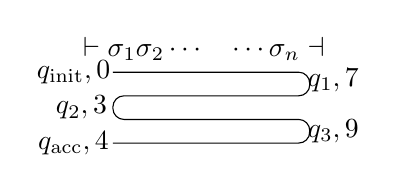
\begin{tikzpicture}
			\node (w) at (0.4,1.8) {$\lmark \sigma_1 \sigma_2\cdots$};
			\node (we) at (2.1,1.8) {$\cdots \sigma_n \rmark$};
			\draw [rounded corners=4pt] (0,1.5) -- (2.5,1.5) -- (2.5,1.2) -- (0,1.2) --
			(0,0.9) -- (2.5,0.9) -- (2.5,0.6) -- (0,0.6);
			\node (qinit) at (-0.5,1.5) {$\initstate,0$};
			\node (q1) at (2.8,1.4) {$q_1,7$};
			\node (q2) at (-0.4,1.05) {$q_2,3$};
			\node (q3) at (2.8,0.75) {$q_3,9$};
			\node (qfin) at (-0.5,0.6) {$\accstate,4$};
		\end{tikzpicture}
		~~
		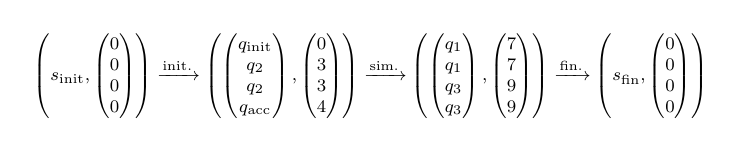
\begin{tikzpicture}[scale=0.8,transform shape]
			\footnotesize
			\node (a) at (0,0) {
				$\left(s_{\textrm{init}},
				\begin{pmatrix}
					0 \\ 0 \\ 0 \\ 0
				\end{pmatrix}\right) \xrightarrow{\text{init.}}
				\left(\begin{pmatrix} \initstate \\ q_2 \\ q_2 \\ \accstate \end{pmatrix},
				\begin{pmatrix} 0 \\ 3 \\ 3 \\ 4 \end{pmatrix}
				\right)
				\xrightarrow{\text{sim.}}
				\left(
				\begin{pmatrix} q_1 \\ q_1 \\ q_3 \\ q_3 \end{pmatrix},
				\begin{pmatrix} 7 \\ 7 \\ 9 \\ 9 \end{pmatrix}
				\right)
				\xrightarrow{\text{fin.}}  \left(s_{\textrm{fin}},
				\begin{pmatrix} 0 \\ 0 \\ 0 \\ 0 \end{pmatrix} \right)$
			};
		\end{tikzpicture}
		\caption{Left: A run of a sweeping 2-OCN. The pairs represent the state and
			counter value at the end of each sweep. Right: The corresponding successful
			run of $\mathcal{V}$.}
		\label{fig:sweeping_runs}
	\end{figure}
	
	We can simulate the entire run of $\cA$ on $w$ using a VASS $\cV$ by,
	intuitively, tracking all the forward sweeps in parallel with all the backward
	sweeps, where for the backward sweeps we simulate the \emph{reverse} 2-OCN of
	$\cA$, denoted $\cA^R$. The latter is a 2-OCN obtained from reversing the
	transitions, as well as negating the counter effects and the head shifts in all
	transitions.  In order to make sure the sweeps concatenate correctly, we guess
	the states and the counter values. Specifically, we proceed as follows.  We
	start by guessing the state in which each backward sweep ends. In this case, a
	successful guess is $(\initstate,q_2,\accstate)$ (note that all guesses must
	start and end in the initial and accepting state). We then guess the counter
	values with which each backward sweep ends. We store two copies of each guess,
	one used to simulate the backward run, and the other to simulate the next
	forward run (except for the last sweep). In our example, the successful guess is
	$(0,3,3,4)$ (where $0$ is the initial counter for the first forward sweep).
	
	At each step, we now nondeterministically guess letters and corresponding
	transitions from $\cA$ for the forward sweep, and from $\cA^R$ for the backward
	sweep. After guessing the correct word $w$ and keeping track of the counters in
	all components, we would then reach the counters $(7,7,9,9)$. Indeed, the
	forward run from $0$ reaches counter $7$, whereas the backward run from $3$
	starts from counter $7$, and hence $\cA^R$ would yield $7$ along the reversal of
	the run. In addition, we track the states of $\cA$ and of $\cA^R$ along each
	run.
	
	The last component of $\cV$ verifies that the concatenation is correct,
	i.e., that each pair of adjacent counters are equal, and that the reached states
	match. The latter is encoded in the states, and the former is tested by
	decreasing both counters together, and checking reachability of $\vec{0}$.
	
	In order to generalize the example above, it is crucial that the number of
	sweeps be \emph{uniformly bounded}. To this end, we observe that if there are
	more than $|Q|$ forward-backward sweeps along a run, then a state is visited
	twice at $\lmark$, i.e., forms a loop. If this loop decreases the counter, then
	there is a shorter run with higher counters, so we need not simulate this former
	run.  If this loop increases the counter, then by repeating it we can obtain an
	arbitrarily high counter. We can then discard the counter and look for a short
	accepting run, based on the 2-NFA obtained from $\cA$, similarly
	to~\cref{sec:2OCN_Bounded_to_VASS_intuitive}.  However,
	unlike~\cref{sec:2OCN_Bounded_to_VASS_intuitive}, we cannot simply simulate the
	2-NFA, since we are committed to a single sweep on the guessed word. In order to
	overcome this, we \emph{initially} guess which state \(q\) will repeat in a positive loop,
	and then simulate a DFA that is
	equivalent~\cite{shepherdson1959reduction,rabin1959finite,vardi1989note} to the
	2-NFA above, starting from state $q$. At the end of the run, we verify using the
	reachability query that the loop is indeed positive.
	%
	Combining these ideas yields a VASS with the conditions above.
	%, 
	%completing the proof. %upper bound of~\cref{lem:Emptiness_Sweeping_Upper_Bound}.
\end{proof}
%
%\subsection{Ackermann-hardness of Emptiness for Sweeping 2-OCN} 
%We complement the upper-bound of~\cref{thm:Emptiness_Sweeping_decidable_ackermann} with a matching lower bound.
\begin{theorem}
	\label{lem:ackermann_hard_sweeping} The emptiness problem for sweeping
	2-OCN is Ackermann-hard.
\end{theorem}
\begin{proof}
	%  \shtodo{figure?}
	We show a reduction from VASS reachability, known to be
	Ackermann-hard~\cite{leroux2022reachability,czerwinski2022reachability}, to
	nonemptiness of sweeping 2-OCN. Specifically, we assume that the
	reachability query is from $(s_1,\vec{0})$ to $(s_2,\vec{0})$, as this
	preserves the hardness.
	
	Consider a VASS $\cV=\tup{S,T}$ of dimension $d$ and configurations
	$(s_1,\vec{0})$ to $(s_2,\vec{0})$.  We construct a sweeping 2-OCN
	$\cA=\tup{Q,T,\Delta,\initstate,\accstate}$ where the alphabet is $T$, i.e., the
	transitions of $\cV$. $\cA$ works as follows: given a word $w\in T^*$, first
	$\cA$ sweeps forward and checks that the states given by the transitions
	follow a run from $s_1$ to $s_2$ in $\cV$ (ignoring the counter values). If
	this fails, $\cA$ rejects.
	
	Next, $\cA$ checks that the counter updates are valid and take the
	configuration from $\vec{0}$ to $\vec{0}$. This is done in two phases. In
	the first phase, $\cA$ makes $d$ forward sweeps, where sweep $i$ simulates
	the $i$-th counter of $\cV$ in the transitions given by $w$, and each
	backward sweep resets the counter to $0$ by negating the effect of the
	transition.  Thus, if the $d$ sweeps complete successfully, we are assured
	that $w$ prescribes a run that reaches from $(s_1,\vec{0})$ to
	$(s_2,\vec{v})$ for some $\vec{v}\ge \vec{0}$.  Then, $\cA$ makes a forward
	sweep while keeping the counter at $0$ and starts the second phase, where we
	perform the same simulation but backwards: we check that the run prescribed
	by $w^R$ (the reverse of $w$) leads from $(s_2,\vec{0})$ to $(s_1,\vec{v'})$
	for some $\vec{v'}\ge\vec{0}$ (note that here we negate the counter
	operations).
	
	The main observation required to complete the proof is that a for a run $\rho$
	of $\cV$ from $(s_1,\vec{0})$ to $(s_2,\vec{v})$ we have that $\rho^R$ (with
	negated counters) is a valid run from $(s_2,\vec{0})$ iff $\vec{v}=0$. This
	follows immediately from the VASS semantics.
	
	We conclude that $L(\cA)\neq \emptyset$ iff $(s_2,\vec{0})$ is reachable from
	$(s_1,\vec{0})$ in $\cV$.
\end{proof}

% \begin{proof}[Proof Sketch (see Appendix~\ref{apx:ackermann_hard_sweeping})]
	% The proof is by reduction from VASS reachability, a problem known to be Ackermann-hard~\cite{leroux2022reachability,czerwinski2022reachability}.
	%   We assume that the VASS reachability query is from $(s_1,\vec{0})$ to
	%   $(s_2,\vec{0})$, as this preserves the hardness.  Consider a VASS
	%   $\cV=\tup{S,T}$ of dimension $d$ and configurations $(s_1,\vec{0})$ to
	%   $(s_2,\vec{0})$.  We construct a sweeping 2-OCN
	%   $\cA=\tup{Q,T,\Delta,\initstate,\accstate}$ where the alphabet is $T$, i.e., the
	%   transitions of $\cV$. Intuitively, $\cA$ works by sweeping forward and
	%   checking that the counter updates are valid in the first counter of $\cV$
	%   alone, using its own counter. Since the transitions are written as the input,
	%   $\cA$ then sweeps back to $\lmark$ while negating the effect of the
	%   transitions, so as to reset the counter. It then repeats this for the other
	%   counters of $\cV$.
	
	%   Note that this only ensures reachability from $(s_1,\vec{0})$ to $(s_2,\vec{v})$ for some $\vec{v}\ge 0$. Therefore, $\cA$ then sweeps forward with counter 0, and repeats the process on the negated-reverse computation of $\cV$.
	% \end{proof}

% Next, $\cA$ checks that the counter updates are valid and take the
% configuration from $\vec{0}$ to $\vec{0}$. This is done in two phases. In
% the first phase, $\cA$ makes $d$ forward sweeps, where sweep $i$ simulates
% the $i$-th counter of $\cV$ in the transitions given by $w$, and each
% backward sweep resets the counter to $0$ by negating the effect of the
% transition.  Thus, if the $d$ sweeps complete successfully, we are assured
% that $w$ prescribes a run that reaches from $(s_1,\vec{0})$ to
% $(s_2,\vec{v})$ for some $\vec{v}\ge \vec{0}$.  Then, $\cA$ makes a forward
% sweep while keeping the counter at $0$ and starts the second phase, where we
% perform the same simulation but backwards: we check that the run prescribed
% by $w^R$ (the reverse of $w$) leads from $(s_2,\vec{0})$ to $(s_1,\vec{v'})$
% for some $\vec{v'}\ge\vec{0}$ (note that here we negate the counter
% operations).

% The main observation required to complete the proof is that a for a run $\rho$
% of $\cV$ from $(s_1,\vec{0})$ to $(s_2,\vec{v})$ we have that $\rho^R$ (with
% negated counters) is a valid run from $(s_2,\vec{0})$ iff $\vec{v}=0$. This
% follows immediately from the VASS semantics.

% We conclude that $L(\cA)\neq \emptyset$ iff $(s_2,\vec{0})$ is reachable from
% $(s_1,\vec{0})$ in $\cV$.
%\end{proof}


\subsection{The Membership Problem for 2-OCN is Polytime}

Recall that by~\cite{chan1987two}, if a 2-OCN $\cA$ has counter updates in
$\{-1,0,1\}$, we can compute in polynomial time (in the description of $\cA$) a
polynomial $p$ such that if a word $w$ is accepted, then it is accepted with a
run of length at most $p(|w|)$.  Unfortunately, this does not carry through to
our setting, where counters are encoded in binary, as the following example shows:
\begin{figure}[ht]
	\vspace*{-20pt}
	\footnotesize \centering
	\vspace{.3cm}
	
	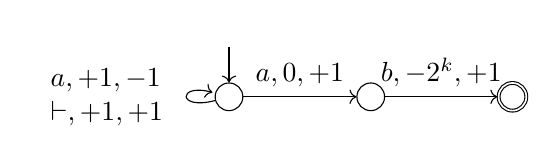
\begin{tikzpicture}[->,node distance=1.8cm, every
		state/.style={minimum size=10pt, inner sep=2pt}]
		\node[state, initial text=,initial above](A){};
		\node[state, right of=A](AA){};
		\node[state, right of=AA,accepting](B){};
		
		\draw (A) edge[loop left] node{$
			\begin{array}{l}
				%\trans{a}{+1}{+1}\\
				\trans{a}{+1}{-1}\\
				\trans{\lmark}{+1}{+1}\\
			\end{array} $} (A) 
		(A) edge[above] node{$\trans{a}{0}{+1}$} (AA)
		(AA) edge[above] node{$\trans{b}{-2^k}{+1}$} (B);
	\end{tikzpicture}
	\vspace{.3cm}
	
	\caption{A 2-OCN $\cA_k$ parameterized by $k\in \bbN$. The word
		$\lmark ab\rmark$ is accepted, but the shortest accepting run is of
		length $2^k+1$, since the counter ``charges'' for $2^k$ steps reading
		only the $\lmark a$ prefix.}
	\label{fig:binary exp run}
\end{figure}

%\pagebreak
Nevertheless, we show that 2-OCN retain efficient membership even with binary
counters:
\begin{theorem}
	\label{thm:membership_PTIME}
	The membership problem for 2-OCN (given a 2-OCN $\cA$ and a word $w$, is $w\in
	L(\cA)$?) is decidable in polynomial time.
\end{theorem}
%\shtodo{Possibly remove proof}
% \begin{proof}[Proof Sketch (see Appendix~\ref{apx:membership})]
	% Similarly to the reasoning in~\cref{sec:2OCN_Bounded_to_VASS_intuitive,sec:sweeping}, we observe that   if an accepting run of $\cA$ on $w$ visits the same state/position pair
	%   $(q,p)$ twice, then if the counter effect between the visits is nonpositive, a shorter accepting run exists, and if the counter effect is positive, then this cycle can be pumped arbitrarily, so that acceptance is dependent only on the 2-NFA obtained by ignoring the counter effects starting from $(q,p)$.
	%   Since the number of state/position pairs is $|w|\cdot |Q|$, it follows that
	%   within $|w|\cdot |Q|+1$ steps we visit a cycle. Similarly,  if an accepting run
	%   exists in the 2-NFA, then there is also one of length at most $|w|\cdot |Q|$.
	
	%   The crux is detecting whether a positive cycle occurs in an accepting run. To this end, we expand the DAG of runs of $\cA$ up to $|w|\cdot |Q|+1$ steps, tracking the maximal counter value attainable for each configuration. Then, for each configuration $(q,p)$ of the DAG, we expand the DAG starting from $(q,p)$, and check if we can reach the same configuration with a higher counter within $|w|\cdot |Q|+1$ steps. This can be done in polynomial time.
	% \end{proof}
% \begin{proof}
	%   Consider a 2-OCN $\cA=\tup{Q,\Sigma,\Delta,\initstate,\accstate}$ and a word
	%   $w\in \Sigma^*$. We implicitly assume that $w$ already includes the end-markers.
	%   Similarly to the reasoning
	%   in~\cref{sec:2OCN_Bounded_to_VASS_intuitive,sec:sweeping}, we observe that
	%   if an accepting run of $\cA$ on $w$ visits the same state/position pair
	%   $(q,p)$ twice, then if the counter effect between the visits is
	%   nonpositive, a shorter accepting run exists, and if the counter effect
	%   is positive, then this cycle can be pumped arbitrarily, so that acceptance
	%   is dependent only on the 2-NFA obtained by ignoring the counter effects starting from $(q,p)$.
	%   Since the number of state/position pairs is $|w|\cdot |Q|$, it follows that
	%   within $|w|\cdot |Q|+1$ steps we visit a cycle. Similarly, in the 2-NFA if an accepting run exists, then there is also one of length at most $|w|\cdot |Q|$.
	
	%   Deciding whether there exists an accepting run in the 2-NFA from $(q,p)$ is straightforward: we keep track of the reachable set of configurations $(q',p')$ at each step of the run, up to $|w|\cdot |Q|$ steps, and if $\accstate$ is reached then the run is accepting.
	
	%   It remains to detect acceptance in the 2-OCN, or to detect a positive cycle. To do so, we proceed as follows. We simulate $\cA$ for $|w|\cdot |Q|$ steps, and for each step $1\le i\le |w|\cdot |Q|$ we store a function $f_i\colon Q\times \{1,\ldots,|w|\}\to \bbN$ that stores for each configuration $(q,p)$ the maximal counter with which $(q,p)$ can be reached after $i$ steps. It is easy to compute $f_i$ from $f_{i-1}$ in polynomial time. Once this simulation is complete, if $\accstate$ does not appear, then we want to look for a positive cycle.
	%   To this end, for each $1\le j\le |w|\cdot |Q|$ and configuration $(q,p)$, we again construct functions $g_j$ similarly to the above, with initial configuration $f_i(q,p)$. If at any point we encounter $(q,p)$ with a counter higher than $f_i(q,p)$, then we have a positive cycle. Otherwise, the word is not accepted.
	
	%   It is easy to verify that all the computations can be carried out in polynomial time.
	% \end{proof}
\begin{proof} 
	Consider a 2-OCN $\cA=\tup{Q,\Sigma,\Delta,\initstate,\accstate}$ and a word
	$w\in \Sigma^*$. We implicitly assume that $w$ already includes the end-markers.
	Similarly to the reasoning 
	in~\cref{sec:2OCN_Bounded_to_VASS_intuitive,sec:sweeping}, we observe that
	if an accepting run of $\cA$ on $w$ visits the same state/position pair
	$(q,p)$ twice, then if the counter effect between the visits is
	nonpositive, a shorter accepting run exists, and if the counter effect
	is positive, then this cycle can be pumped arbitrarily, so that acceptance
	is dependent only on the 2-NFA obtained by ignoring the counter effects starting from $(q,p)$.
	Since the number of state/position pairs is $|w|\cdot |Q|$, it follows that
	within $|w|\cdot |Q|+1$ steps we visit a cycle. Similarly, in the 2-NFA if an accepting run exists, then there is also one of length at most $|w|\cdot |Q|$.
	
	Deciding whether there exists an accepting run in the 2-NFA from $(q,p)$ is straightforward: we keep track of the reachable set of configurations $(q',p')$ at each step of the run, up to $|w|\cdot |Q|$ steps, and if $\accstate$ is reached then the run is accepting.
	
	It remains to detect acceptance in the 2-OCN, or to detect a positive cycle. To do so, we proceed as follows. We simulate $\cA$ for $|w|\cdot |Q|$ steps, and for each step $1\le i\le |w|\cdot |Q|$ we store a function $f_i\colon Q\times \{1,\ldots,|w|\}\to \bbN$ that stores for each configuration $(q,p)$ the maximal counter with which $(q,p)$ can be reached after $i$ steps. It is easy to compute $f_i$ from $f_{i-1}$ in polynomial time. Once this simulation is complete, if $\accstate$ does not appear, then we want to look for a positive cycle.
	To this end, for each $1\le j\le |w|\cdot |Q|$ and configuration $(q,p)$, we again construct functions $g_j$ similarly to the above, with initial configuration $f_i(q,p)$. If at any point we encounter $(q,p)$ with a counter higher than $f_i(q,p)$, then we have a positive cycle. Otherwise, the word is not accepted.
	
	It is easy to verify that all the computations can be carried out in polynomial time.
\end{proof}



\section{On the Semilinearity of 2-OCN Languages}
\label{sec:semilinear}
\mysubparagraph{Preliminaries.}  Emptiness decidability has been historically
intimately tied to \emph{semilinearity}.  A set \(E \subseteq \mathbb{N}^d\) is semilinear if it is
expressible in first-order logic with addition (there are many equivalent
definitions and we will not need a specific one).  The \emph{Parikh image} of a
language \(L\) over an alphabet \(\{a_1, \ldots, a_k\}\) is the set of vectors
\((n_1, \ldots, n_k)\) such that there is a word in \(L\) with precisely \(n_i\) letters
\(a_i\) (in any order), for all \(i\).  In other words, the Parikh image counts the
number \(|w|_\ell\) of times each letter \(\ell\) appears in a word \(w \in L\), resulting in
a set of vectors in \(\mathbb{N}^{|\Sigma|}\).  A class of languages is \emph{semilinear} if for
any language \(L\) in that class, the Parikh image of \(L\) is semilinear.  In that
case, if there is an algorithmic way to obtain a representation of that
semilinear set from a representation of \(L\), then one can check whether
\(L = \emptyset\), since satisfiability is decidable for first-order logic with
addition~\cite{berman1980complexity}.

\mysubparagraph{General 2-OCN.}  Since the emptiness problem is undecidable for
2-DOCN, it is an unsurprising fact that there are nonsemilinear 2-DOCN languages
(e.g., \(\{(a^n\#)^n \mid n > 1\}\)).  A tantalizing question surging from the study in~\cref{sec:bounded_languages} is: \emph{Are all 2-OCN bounded languages semilinear?}  
For 2-DOCN, it is proved in~\cite{miyano1982two} that this is indeed the case. For 2-OCN, it is likely that a proof of this statement would provide an alternative proof to \Cref{thm:emptiness_bounded_decidable}.  We conjecture that, indeed, 2-OCN
are in good company with a wealth of computational models whose bounded
languages are precisely those with a semilinear Parikh image.  We come short of
showing this, but prove, using the construction
of~\cref{sec:2OCN_Bounded_to_VASS_intuitive} and a result
of~\cite{hauschildt1994petri}, that:
\begin{theorem}
	\label{thm:singleton_alphabet_semilinear} For any 2-OCN $\cA$ with \(L(\cA) \subseteq
	a_1^*a_2^*\cdots a_k^*\) and for any \(\Gamma \subseteq \{a_1, a_2, \ldots, a_k\}\), the set $\left\{ \sum_{\ell \in \Gamma}
	|w|_\ell \mid w \in L(\cA)\right\}\subseteq \bbN$ is effectively semilinear.
\end{theorem}
\begin{proof} In~\cite[Corollary 4.3]{hauschildt1994petri} the following is
	shown.\footnote{In~\cite{hauschildt1994petri} the result is phrased for Petri
		Nets, but the equivalence between Petri Nets and VASS gives a straightforward
		translation.  In~\cite{kleinebuning1989}, a slightly weaker result is
		presented in the language of VAS.} Given a VASS $\cV=\tup{S,T}$ of dimension
	$d$ and two states $s_1,s_2$, consider the set $\cR_{s_1,s_2}\subseteq \bbN^d\times \bbN^d\times
	\bbN^T$ such that $(\vec{p},\vec{p'},\vec{t})\in \cR_{s_1,s_2}$ iff
	$(s_2,\vec{p'})$ is reachable from $(s_1,\vec{p})$ via a run $\rho$ that takes
	transition $\tau$ exactly $\vec{t}(\tau)$ times. Then the image of every morphism
	$\pi\colon \cR_{s_1,s_2}\to \bbN$ is effectively semilinear.
	
	In our setting, take $\cV$ to be the VASS obtained
	in~\cref{sec:2OCN_Bounded_to_VASS_intuitive} with the states
	$s_{\textrm{init}}, s_{\textrm{fin}}$ and $\vec{p}=\vec{p'}=\vec{0}$. Let
	$\pi$ be the morphism that counts the number of transitions used to initialize
	$n_i$ for all $a_i \in \Gamma$, and recall that by the correctness of the
	construction of $\cV$, we have that along a run from
	$(s_{\textrm{init}},\vec{0})$ to $(s_{\textrm{fin}},\vec{0})$, the value of
	$n_i$ after the Initialization Component corresponds to the length of the
	$a_i$ segment in an accepted word.  Then, \cite[Corollary
	4.3]{hauschildt1994petri} readily shows that the set
	$\left\{\sum_{a_i \in \Gamma} n_i \mid a_1^{n_1}\cdots a_k^{n_k}\in L(\cA)\right\}$ is effectively
	semilinear.
	% 
	% If \(\cA\) is sweeping, a similar approach relying on counting the transitions
	% that read the letters in \(T\) yields the result.
\end{proof}
The previous theorem implies that 2-OCN languages over a singleton alphabet are
semilinear. In addition, we have the following:
\begin{corollary}
	\label{cor:2DOCA_not_2OCN}
	The languages \(\{0^n 1^{n^2} \mid n \geq 1\}\) and \(\{0^n1^{2^n} \mid n \geq 1 \}\), known
	to be 2-DOCA languages~\cite{petersen1994two}, are not 2-OCN languages.
\end{corollary}

\mysubparagraph{Sweeping 2-OCN.} 
%\shtodo{not sure about the ``seemingly'' below.}
%We note that \Cref{thm:singleton_alphabet_semilinear} does apply to sweeping 2-OCN without the bounded language restriction, with a similar proof, seemingly indicating that sweeping 2-OCN languages are always semilinear.  However:
We note that \Cref{thm:singleton_alphabet_semilinear} also applies to sweeping 2-OCN without the bounded language restriction, with a similar proof. 
\begin{theorem}
	\label{thm:singleton_alphabet_semilinear_sweeping} For any sweeping 2-OCN $\cA$ over $\Sigma$ and \(\Gamma \subseteq \Sigma\), $\left\{ \sum_{\ell \in \Gamma}
	|w|_\ell \mid w \in L(\cA)\right\}$ is effectively semilinear.
\end{theorem}
However, unlike the case of bounded languages, here we can show that the Parikh image of sweeping 2-OCN language are not always semilinear.
\begin{proposition}
	\label{prop:non_semilinear_sweeping}
	There are nonsemilinear languages recognized by sweeping 2-DOCN.
\end{proposition}
\begin{proof}
	Consider the Dyck language over \(\{a, b\}\), i.e., well-parenthesized
	expressions where \(a\) corresponds to an opening parenthesis and \(b\) to a
	closing one.  Write \(P\) for the prefixes of that language.  Clearly, \(P\) is a
	1-DOCN language.  Write \(P'\) for the language \(P\) where \(a\) and \(b\) swap
	roles.  We can construct a sweeping 2-DOCN that recognizes \(K = P \cap a^*P'\)
	using the closure of 2-DOCN under intersection~\cite{miyano1982two} (which preserves the sweeping property).  
	In any word \(w\) in \(K\), if \(n\) is the length of the first block of
	\(a\)'s, then \(0 \leq |w|_a - |w|_b \leq n\).  Finally, using a few more sweeps, we can
	express:
	\[
	L = \{c^n \# w \mid w \in K \land w \in a^n(b^+a^+)^{n-1}b^n \}.
	\]
	Indeed, this requires checking that the number of $c$'s is equal to the number
	of $a$'s in the first block, the number of $b$'s in the last block, and the
	number of $ab$ infixes.
	
	Now, for a fixed value \(n\), the longest word in \(L\) that can appear after \(c^n\#\) is
	\((a^nb^n)^n\), of length \(2n^2\), showing that this language is not semilinear.
\end{proof}

We will show, in \Cref{sec:nondet_vs_det}, that there is a 1-OCN language (thus
a sweeping 2-OCN language) this is not expressible using a 2-DOCN.  Conversely,
\Cref{prop:non_semilinear_sweeping} provides an easy way to show that:
\begin{corollary}
	There is a 2-DOCN language that is not expressible using a sweeping 2-OCN.
\end{corollary}
\begin{proof}
	\def\ub{\underline{b}}%
	\def\ss{\,\#\,}%
	Consider the language \(L\) over the alphabet \(\{a, b, c, \#, \ub, x\}\) defined
	as:
	\[L = \{a^n\ss b^mx^m\ss\ub^mx^{2m}\ss\ub^mx^{3m}\ss\cdots\ss\ub^mc^{nm} \mid n, m > 0\}\]
	By applying the morphism $h\colon \Sigma^*\to \Sigma^*$ that erases $\ub,\#$, and $x$, we
	have $h(L) = \{a^nb^mc^{nm}\}$, which can be seen as multiplication.
	
	The language $L$ is recognizable by a 2-DOCN $\cA$ by repeatedly using a
	similar approach to~\cref{xmp:aNbN}:
	\begin{compactitem}
		\item Check that the input has the form \(a^*\#b^*(x^*\#\ub^*)^*c^*\),
		\item Check that the number of \(a\)'s is the same as the number of \(\#\)'s,
		% (i.e., the \(c\)'s appear in the \(n\)-th block delimited by \(\#\));
		\item Check that the first sequence of \(\ub\)'s is as long as the sequence of \(b\)'s,
		\item Check that the lengths of all sequences of \(\ub\)'s are equal, by checking that each neighboring sequence
		\(\#\ub^ix^*\#\ub^jx^*\) satisfies \(i = j\),
		\item Check for each sequence \(x^i\#\ub^mx^j\) that \(i + m = j\), and the same
		for the last segment where $x$ is replaced with $c$.
	\end{compactitem}
	This 2-DOCN proceeds segment by segment, always making sure that the number of
	$x$'s increases by exactly $m$. This, together with the initial test that the
	number of segments is $n$, forces the number of $c$'s to be exactly $nm$.
	
	However, the lengths of words in this language do not form a semilinear set,
	so by~\cref{thm:singleton_alphabet_semilinear_sweeping} it cannot be
	recognized by a sweeping 2-OCN.
\end{proof}

Over bounded languages, the following exact characterization holds:
\begin{theorem}
	\label{thm:bounded_sweeping_equiv_semilinear} A bounded language is recognized by a sweeping
	2-OCN iff it is semilinear.
\end{theorem}
\begin{proof}
	The fact that any semilinear bounded language can be expressed with a sweeping
	2-OCN is easily deduced from the fact that semilinear sets are those
	expressible with \emph{quantifier-free} first-order formulas with addition,
	order, and modulo.  Putting such a formula in DNF, we simply need to guess
	which conjunction is to hold, and the conjunction can be checked by a sweeping
	2-DOCN using the closure of 2-DOCN under intersection~\cite{miyano1982two} (which preserves the sweeping property).
	
	We turn to the fact that bounded languages expressed by sweeping 2-OCN are
	semilinear.  We split the proof into two parts.
	
	\mysubparagraph{Constant number of sweeps.}  Let us first assume that the
	sweeping 2-OCN \(\cA\) executes a constant number of sweeps, say \(C\), with
	\(C\) odd, for each input word (we assume here that the machine ends at the
	right end-marker).  With \(L(\cA) \subseteq a_1^*\cdots a_k^*\), consider the following
	transformation that produces a word over the alphabet
	\(\Gamma = \{a_{i,j} \mid 1 \leq i \leq C \land 1 \leq j \leq k\}\):
	\[w = a_1^{n_1}\cdots a_k^{n_k} \quad \leadsto \quad w' = a_{1,1}^{n_1}\cdots a_{1,k}^{n_k} \,\#\,
	a_{2,k}^{n_k}\cdots a_{2,1}^{n_1} \,\#\, \cdots \,\#\, a_{C,1}^{n_1}\cdots
	a_{C,k}^{n_k}.\]%
	That is, the input is replicated \(C\) times, with every other copy reversed,
	and each copy on its own alphabet.  Let us call \(w'\) the \emph{replica} of
	\(w\).  Since \(\cA\) makes at most \(C\) sweeps, we can build a 1-OCN \(\cB\) that
	reads the replica of any word \(w \in a_1^*\cdots a_k^*\) and accepts if and only if
	\(w\) is accepted by the 2-OCN (and the input is of the format \(R =
	a_{1,1}^*\cdots a_{1,k}^*\#a_{2,k}^*\cdots a_{2,1}^*\#\cdots\) \(\# a_{C,1}^*\cdots a_{C,k}^*\)). 
	Naturally, \(\cB\) also accepts words that are
	\emph{not} replicas. 
	%We can however force \(\cB\) to accept only words in \(R = a_{1,1}^*\cdots a_{1,k}^*\#a_{2,k}^*\cdots a_{2,1}^*\#\cdots\# a_{C,1}^*\cdots a_{C,k}^*\). 
	
	We circumvent this problem by using an ``external'' semilinear set, as follows. Let
	\(E\) be the Parikh image of the language where for all \(i\), each \(a_{\bullet,i}\)
	appears the same number of times; clearly, a word in \(R\) is a replica iff its
	Parikh image is in \(E\).  Since \(\cB\) is a 1-OCN language (and in particular context-free), the Parikh image \(F\)
	of its language is semilinear by Parikh's Theorem~\cite{parikh66}.  
	It is then easy to check that \(E \cap F\) is exactly
	the set of Parikh images of replicas of words in \(L(\cA)\), showing that the
	Parikh image of \(L(\cA)\) itself is semilinear (as a projection of the former).
	
	\newcommand{\ifemptyTF}[3]{%
		\if\relax\detokenize{#1}\relax #2\else #3\fi
	}
	\makeatletter
	\def\@claplines#1\\#2\;{%
		\mathclap{#1}%
		\ifemptyTF{#2}{}{\\\@claplines #2\;}%
		\@gobble\fi % for alignment
	}
	\def\claplines#1{\@claplines #1\\\;}
	\makeatother
	\newcommand{\ind}[3][\bigg]{\underset{\substack{#1\uparrow\\\claplines{#3}}}{#2}}
	\def\pp{\texttt{+}}\def\mm{\texttt{-}}
	
	\mysubparagraph{Any number of sweeps.}
	If \(\cA\) is sweeping but does not do a constant number of sweeps for each
	input, we adapt the recurring idea of \Cref{sec:bounded_languages,sec:sweeping}.  Let \(k\) be the number of
	states of \(\cA\).  After \(2k+1\) sweeps, a state is repeated at the left end-marker; if
	the counter effect between the two repetitions is nonpositive,
	then that run is not useful for acceptance, and can be disregarded.  
	If the counter \emph{increases}, then it can be increased 
	arbitrarily, and the behavior of the 2-OCN is the same as a 2-NFA \(\cN\) from
	that point on.  Consider the 1-OCN \(\cB\) constructed above,
	with \(C = 2k+1\).  We can additionally have \(\cB\) guess the state that repeats,
	if any, and check that it indeed repeats.  Next, \(\cB\) assumes that the
	counter strictly increases in the repetition, and branches into a DFA for
	\(\cN\).  In order to ``kill'' the runs of \(\cB\) where this assumption is
	incorrect, any transition that \(\cB\) takes, in between the first and second
	appearance of the repeated state, should be followed by input symbols
	indicating the counter effect, increasing ($\pp^*$) or decreasing ($\mm^*$),
	and by how much. $\cB$ then verifies that the correct effect is matched to the
	transition of $\cA$ it guesses.  For instance, \(\cB\) may read the following
	replica of \(aabbbc\) with extra counter information (here the original alphabet
	is \(\{a, b, c\}\) and the replica alphabet has \(1, \ldots, 5\) as indices):
	% 
	\[\underbrace{a_1a_1b_1b_1b_1c_1 \# c_2b_2b_2b_2a_2a_2}_{\cB\text{ simulates
			two sweeps of $\cA$}}
	\ind{\#}{\cB\text{ guesses state repetition}}
	\underbrace{a_3\pp\pp a_3\pp b_3\mm b_3\pp b_3\mm c_3\pp \# c_4\mm b_4\pp b_4\pp
		b_4\mm a_4\mm a_4\mm }_{%
		\substack{\claplines{\text{counter updates appear in input}\\
				\text{showing action of $\cA$'s transitions}}}}
	\ind{\#}{\cB\text{ checks state repetition}\\
		\text{and assumes that counter increased}}
	\underbrace{a_5a_5b_5b_5b_5c_5 \#}_{\text{A DFA for $\cN$ is ran}}\]
	% 
	% 
	As mentioned, this modified version of \(\cB\) may jump into a DFA for \(\cN\)
	when it should not.  However, we can augment the external semilienar set \(E\), checking that the input word is a replica, to also check that %if a state repetition is guessed,
	%then 
	the number of \(\pp\) is strictly greater than the number of \(\mm\).  This
	corresponds to the counter updates between the state repetitions having a
	strict positive impact, and that \(\cB\) correctly jumps into \(\cN\)'s
	simulation.  
	To conclude, let again \(F\) be the (semilinear) Parikh image of
	the language of \(\cB\).  The vectors in \(E \cap F\) correspond precisely to the
	replicas (with possibly explicit counter updates) that are accepted by \(\cA\),
	hence the language of \(\cA\) is semilinear.
\end{proof}

\section{2-DOCN  vs 1-OCN: A Pumping Lemma for  2-DOCN}
\label{sec:nondet_vs_det}
In~\cite{chan1987two} it is shown that the language $\{a^nb^m\mid n\neq m\}$ is 2-OCN
recognizable but not 2-DOCN recognizable. We strengthen this result in two
directions: first we present a general pumping lemma that we can then use to
establish that various languages are not 2-DOCN-recognizable. Second, using our
lemma we are able to find a language that is not 2-DOCN recognizable, but is
already 1-OCN recognizable. This shows that nondeterminism can be used to
compensate for two-wayness, in some settings.
\begin{lemma}\label{lem:2DOCN_pump}
	Let $\Sigma$ be an alphabet and $a\in \Sigma$. For every 2-DOCN-recognizable language
	\(L\subseteq \Sigma^*\) there exists \(K \in \bbN\) such that for every $x,y\in \Sigma^*$, if \(xa^Ky \notin
	L\) then there exists $K'\neq K$ such that \(xa^{K'}y \notin L\) as well.
\end{lemma} 
We give a rough sketch of the main ideas of the proof, see Appendix~\ref{apx:proofs_nondet_vs_det} for the complete arguments and definitions.
%
%We prove \cref{lem:2DOCN_pump} in the remainder of this
%section. Missing proofs are in Appendix~\ref{apx:proofs_nondet_vs_det}.
Consider a 2-DOCN $\cA=\tup{Q,\Sigma,\Delta,\initstate,\accstate}$, and think of $K$ as some large constant.
%and denote by $M=|Q|$ the number of states in $\cA$. 
Our goal is to devise a way to pump certain infixes of a word $xa^Ky$, so that we can reason about the resulting run of $\cA$ on it. 
Naturally, the challenge lies in synchronizing the behaviors of forward and backward head movements in the run.

%We set the bound $K$ prescribed in~\cref{lem:2DOCN_pump} to be
%$K=M+(M+1)^{2(M+1)}+1+M$, and 
We think of the $a^K$ infix as partitioned to three parts: two short $a^{|Q|}$ segments referred to as \emph{outer left $a$'s} and \emph{outer right $a$'s}, and a long $a^{K-2|Q|}$ segment in the middle, called the \emph{inner $a$'s}. We depict the word $xa^Ky$ as \emptytape, with the grayed area representing the inner $a$'s, and the vertical lines marking the end of $x$ and the beginning of $y$.

We then consider the form of the run of $\cA$ on $xa^Ky$. Specifically, we divide runs according to whether they cross into the inner $a$'s. We show that runs that do reach the inner $a$'s, must continue to the end of the tape (either from right or left). Runs that do not cross the inner $a$'s must therefore get stuck in a small part of the tape. By depicting runs as
going from top to bottom upon head reversal, we have e.g., the type \leftcrossing which
depicts runs going left, and \rightcrossing depicts runs going right. The possible types of runs are then \emph{left loop} (\leftloop), \emph{left sink} (\leftsink), \emph{left crossing} (\leftcrossing) and their right counterparts. Each type signifies a specific behavior of the runs, e.g., whether they repeat a state, or stop due to the counter becoming negative.

We define a \emph{round trip} to be a concatenation of runs of the form \leftloop\rightcrossing\rightloop\leftcrossing, and show that either (1) $\cA$ has a run on $xa^Ky$ with many round-trips, or (2) it has a run with a few round trips that gets stuck in a loop, or (3) its maximal run has few round trips and ends with the counter becoming negative. 
We then provide pumping arguments according to each type of run. 

A crux of the proof lies in handling Form (3) above. The main idea is the following: consider a run with several round-trips that ends due to a counter becoming negative. Since the inner $a$'s are a long infix, we can find two indices that are visited with the same sequence of states in the round trips. We can then attempt to ``pump'' or ``cut'' the infix between these indices, but this may cause the counter to ultimately increase, thus yielding an accepting run from a previously-rejecting one. 
We therefore carefully analyze the effect of the counter between these two indices on each pass of the form \rightcrossing or \leftcrossing. If at any point the cumulative sum of effects is negative, we can pump the run enough so that the counter ultimately becomes negative, and the word is not accepted. 
Otherwise, all the cumulative sums are non-negative, in which case we can cut the cycle, causing the counter to either become negative or to complete the run in the same state as the original run, which is not accepting. The precise details are involved and appear in Appendix~\ref{apx:proofs_nondet_vs_det}.


% We start by observing
% that if the run of $\cA$ never moves the head beyond $x$, then the lemma is
% trivial. We therefore assume that the head does go beyond $x$, and we start all
% our reasoning assuming that this prefix of the run was already taken, i.e., that
% the head now lies on the last letter of $x$.

% \begin{definition}
	%   \label{def:run_types} Consider a run $\rho=(q_1,c_1,p_1),\ldots,(q_n,c_n,p_n)$. We say
	%   that $\rho$ is:
	%   \begin{compactitem}
		%   \item a \emph{left loop}, denoted $\rho\in \leftloop$, if $p_1=p_n=|x|$ and for every
		%     $1\le i\le n$ we have $p_i\le |x|+K$.
		%   \item a \emph{right loop}, denoted $\rho\in \rightloop$ if $p_1=p_n=|x|+K+1$ and for
		%     every $1\le i\le n$ we have $p_i>|x|$.
		%   \item a \emph{left sink}, denoted $\rho\in \leftsink$ if $p_1=|x|$, for every $1\le i\le
		%     n$ we have $p_i\le |x|+K$ and there exist $1\le j< n$ such that $q_j=q_n$ and
		%     $p_j=p_n$.
		%   \item a \emph{right sink}, denoted $\rho\in \rightsink$ if $p_1=|x|+K+1$, for every
		%     $1\le i\le n$ we have $p_i>|x|$ and there exist $1\le j< n$ such that $q_j=q_n$ and
		%     $p_j=p_n$.
		%   \item a \emph{right crossing}, denoted $\rho\in \rightcrossing$ if $p_1=|x|$,
		%     $p_n=|x|+K+1$, for every $1< i< n$ we have $|x|<p_i<|x|+K+1$.
		%   \item a \emph{left crossing}, denoted $\rho\in \leftcrossing$ if $p_1=|x|+K+1$,
		%     $p_n=|x|$, for every $1< i< n$ we have $|x|<p_i<|x|+K+1$.
		%   \item a \emph{round trip} if $\rho=l\cdot c_r\cdot r\cdot c_l$ with\footnote{We often
			%       concatenate runs $\alpha\cdot \beta$ where $\alpha$ ends with the same configuration $\beta$ starts
			%       with. In such cases, the concatenation means that we omit the overlapping
			%       configuration.} $l\in \leftloop$, $c_r\in \rightcrossing$, $r\in \rightloop$ and
		%     $c_l\in \leftcrossing$.
		%   \end{compactitem}
	% \end{definition}
% \begin{remark}[Drawing Convention]
	%   Our convention for depicting run types uses \emptytape to depict the word
	%   $xa^Ky$, with the grayed area representing the inner $a$'s, and the vertical
	%   lines marking the end of $x$ and the beginning of $y$. Runs are depicted as
	%   going from top to bottom upon head reversal, for instance \leftcrossing
	%   depicts runs going left, and \rightcrossing depicts runs going right. We
	%   remark that the drawings serve no formal role, only a convention to assist the
	%   naming of run types.
	% \end{remark} Our first claim is that if the run of $\cA$ moves from $x$ and
% crosses from the outer left $a$'s to the inner $a$'s, then the run must complete
% the traversal of $a$'s and cross over to $y$ before seeing $x$ again (and dually
% for right-to-left runs).  Intuitively, this is because $\cA$ is deterministic
% and therefore cannot read many $a$'s before entering a right-traversing cycle.

% \begin{lemma}\label{lem:inner_implies_crossing}
	%   Consider a run $\rho=(q_1, c_1, p_1)\cdots (q_n, c_n, p_n)$. If $\rho\in \leftloop$ (left
	%   loop) or $\rho\in \leftsink$ (left sink), then $p_i \leq |x|+M$ for all $1\leq i \leq n$.
	%   Similarly, if $\rho\in \rightloop$ (right loop) or $\rho\in \rightsink$ (right sink),
	%   then $p_i \geq |x|+K+1-M$ for all $1\leq i \leq n$.
	% \end{lemma}

% % \begin{proof}
	% %   Consider the case where $\rho\in \leftloop$, and assume by way of contradiction
	% %   that $\rho$ crosses to position $|x|+(M+1)$. Then the infix of $\rho$ before the
	% %   first time it reaches position $|x|+(M+1)$ contains a sequence of at least
	% %   $M+1$ configurations within the left-outer $a$, upon which the head moves to
	% %   the right.
	% %   Thus, $\rho$ has a cycle from some state $q$ upon reading $a$'s that moves the head some $j$ positions to the right. This cycle is then repeatedly taken until a letter other than $a$ is
	% %   encountered, which only occurs on $y\rmark$. Thus, $\rho$ must visit position
	% %   $|x|+K$ before reaching position $0$ again, in contradiction to it being a
	% %   left-loop.
	
	% %   The analysis for the remaining three types of runs is similar.
	% % \end{proof}

% We now turn to identifying forms of runs of $\cA$ on $xa^Ky$, based on their
% decomposition to round trips (see~\cref{def:run_types}). Recall that while $\cA$
% is deterministic, it may have many (possibly infinitely many) runs on $xa^Ky$,
% ordered by the prefix relation.
% \begin{definition}
	%   \label{def:run_forms} Consider a run $\rho$ of $\cA$ on $xa^Ky$. We say that $\rho$
	%   has:
	%   \begin{compactenum}
		%   \item \emph{Form 1: Many round trips} if $\rho=r_1\cdot r_2,\cdots r_{M+1}$ for round
		%     trips $r_1,\ldots,r_{M+1}$.
		%   \item \emph{Form 2: Few round trips and a sink} if $\rho=r_1\cdot r_2,\cdots r_m\cdot I$ for
		%     round trips $r_1,\ldots,r_m$ where $m\le M$ and $I$ is either $\leftsink$ (left sink)
		%     or $I=l\cdot c_r\cdot d$ with $l\in \leftloop$, $c_r\in \rightcrossing$ and
		%     $d\in \rightsink$.
		%   \item \emph{Form 3: Few round trips cut short} if $\rho=r_1\cdot r_2,\cdots r_m\cdot C$ for
		%     round trips $r_1,\ldots,r_m$ where $m\le M$ and $C$ is a prefix of a round trip.
		%   \end{compactenum}
	% \end{definition}

% Intuitively, if $\cA$ has a long-enough run on $xa^Ky$, then either it contains many round trips, or it gets stuck in a loop. Otherwise, the longest run is cut short by the counter becoming negative. We thus have the following.
% \begin{lemma}\label{lem:run_forms}
	%   Let $\Upsilon$ be the set of run-prefixes of $\cA$ on $xa^Ky$, then either there is a
	%   run $\rho\in \Upsilon$ of Form 1 or of Form 2, or $\Upsilon$ is finite and the maximal-length run
	%   in $\Upsilon$ is of Form 3.
	% \end{lemma}
% % \begin{proof}
	% %   Recall that $\cA$ does not accept $xa^Ky$, and therefore there is no accepting
	% %   run.  The main observation required in the proof is that
	% %   by~\cref{lem:inner_implies_crossing}, if a left loop $\leftloop$ is longer
	% %   than $M(|x|+M)+1$, then it has a prefix that is a left sink
	% %   $\leftsink$. Indeed, a left loop must stay within the outer-left $a^{M}$, and
	% %   uses at most $M$ states. Similarly, a right loop longer than $M(|y|+M)+1$ has
	% %   a prefix that is a right sink.  Still by~\cref{lem:inner_implies_crossing}, a
	% %   run that starts at position $|x|$ (resp. $K+1$) and reaches the inner $a$'s is
	% %   a right crossing (resp. left crossing).
	
	% %   Therefore, runs from position 0 start as a (possibly empty) left loop
	% %   $\leftloop$, followed by a right crossing $\rightcrossing$, then a right loop
	% %   $\rightloop$, then a $\leftcrossing$. This repeats until either the run cannot
	% %   continue due to the counter becoming negative, or due to one of the loops
	% %   becoming a sink.
	
	% %   The lemma now readily follows: if $\Upsilon$ has a long enough run of Form 1, we are
	% %   done.  Otherwise all runs in $\Upsilon$ have at most $M$ round trips. Then, either
	% %   $\Upsilon$ has a run that ends with a left or right sink, or $\Upsilon$ is finite and the
	% %   maximal run ends due to the counter becoming negative (i.e., ends with a
	% %   prefix of a round trip).
	% % \end{proof}

% Having established the form of runs, we now turn to our main pumping
% argument. To this end, we identify within the inner $a$'s two positions that
% form a ``cycle'' with respect to left and right crossings.

% Let $c$ be a left or right crossing. We say that two positions $p_1,p_2$
% are \emph{$c$-matching positions} if $|x|+M+1 \leq p_1<p_2 \leq |x|+K-M$ (i.e., these
% two positions are in the inner $a$'s) and the first time positions $p_1,p_2$
% occur in $c$, they occur with the same state.

% We extend the definition to prefixes of $c$: for a prefix $c'\pref c$, we say
% that $|x|+M+1 \leq p_1<p_2 \leq |x|+K-M$ are $c'$-matching positions if either both
% positions occur in $c'$ and appear for the first time with the same state, or
% both positions do not occur in $c'$.

% Next, we lift the definition to concatenations of runs: for a run $\rho$ that is a
% concatenation of the types in~\cref{def:run_types} and prefixes thereof, we say
% that $|x|+M+1 \leq p_1<p_2 \leq |x|+K-M$ are matching positions if they are matching
% for every crossing (or prefix of a crossing) in $\rho$.  In particular, for a round
% trip $R=l\cdot c_r\cdot r\cdot c_l$, positions $p_1,p_2$ are matching if they are matching
% for both $c_r$ and $c_l$.

% Since matching positions are, intuitively, a cycle in the run, we can either pump their respective infix or cut it, while the corresponding run is pumped or cut similarly, up to the counter values. That is, the counter may become negative due to pumping or cutting, or it could have previously been negative and after pumping allows the run to continute. This is captured in the following.

% \begin{lemma}
	%   \label{lem:matching_positions_are_pumpable} Let $\rho$ be a run of $\cA$ on
	%   $xa^Ky$ in one of the Forms of~\cref{def:run_forms}, and let $|x|+M+1\le
	%   p_1<p_2\le |x|+K-M$ be matching positions for $\rho$. Let $w^+=xa^{K+(p_2-p_1)}y$
	%   and $w^-=xa^{K-(p_2-p_1)}y$, then there are runs $\rho^+$ and $\rho^-$ of $\cA$
	%   on $w^+$ and $w^-$, respectively, such that each of them either ends in the
	%   same state as $\rho$, or ends due to the counter becoming negative.
	% \end{lemma}
% % \begin{proof}
	% %   We prove the claim for a single round trip $R=l\cdot c_r\cdot r\cdot c_l$ where
	% %   $l\in \leftloop$, $c_r\in \rightcrossing$, $r\in \rightloop$ and
	% %   $c_l\in \leftcrossing$. The claim follows inductively for a concatenation of
	% %   round trips, and is analogous for the suffixes of Forms 2 and 3
	% %   in~\cref{def:run_forms}.
	
	% %   We start with $w^+=xa^{K+(p_2-p_1)}y$.  Denote $R=l \cdot c_{r1}c_{r2}c_{r3} \cdot r \cdot
	% %   c_{l1}c_{l2}c_{l3}$, such that $c_r$ is split into three parts -- before the
	% %   first occurrence of $p_1$, between the first occurrence of $p_1$ and the first
	% %   occurrence of $p_2$, and after the first occurrence of $p_2$. Similarly, $c_l$
	% %   is split so that $c_{l1}$ is before the first occurrence of $p_2$ (since this
	% %   is a left crossing), $c_{l2}$ is between $p_2$ and the first occurrence of
	% %   $p_1$, and $c_{l3}$ is the rest.
	
	% %   For a run infix $\beta$, we denote by $\beta^{+t,+t'}$ the run obtained from $\beta$ by
	% %   offsetting each configuration $(q,c,p)$ to $(q,c+t,p+t')$.  We now consider
	% %   the run
	% %   \[ l\cdot c_{r1}\cdot c_{r2}\cdot (c_{r2}\cdot c_{r3}\cdot r\cdot c_{l1}\cdot
	% %   c_{l2})^{+\eff(c_{r2}),+(p_2-p_1)}\cdot (c_{l2}\cdot
	% %   c_{l3})^{+\eff(c_{r2})+\eff(c_{l2}),+0}
	% %   \]
	% %   Observe that up to the counter updates, this is a run of $\cA$ on
	% %   $w^+$. Indeed, since $p_1$ and $p_2$ are matching positions, then we can take
	% %   in $p_2$ the same transitions of $c_{r2}$, again reaching the same initial
	% %   state of $c_{r3}$. Moreover, since $p_1,p_2$ are in the inner
	% %   $a$'s,~\cref{lem:inner_implies_crossing} guarantees that within the pumped
	% %   infix $c_{r2}$, the head does not reach positions $|x|$ nor $|x|+K+1+(p2-p1)$
	% %   (otherwise this would also happen before pumping). Similar arguments apply for
	% %   the left crossing.  Thus, either this is a run on $w^+$ ending in the same
	% %   state and position as $\rho$, or a prefix of this run ends due to the counter
	% %   becoming negative.
	
	% %   Similarly, for $w^-$ we obtain the run
	% %   \[ l\cdot c_{r1}\cdot (c_{r3}\cdot r\cdot c_{l1})^{-\eff(c_{r2}),-(p_2-p_1)}\cdot
	% %   c_{l3}^{-\eff(c_{r2})-\eff(c_{l2}),+0}
	% %   \]
	% %   and again, similar consideration to~\cref{lem:inner_implies_crossing} show
	% %   that upon reading $c_{r3}$ the run does not reach position 0 before proceeding
	% %   to $r$.
	% % \end{proof}

% We are now ready to complete the proof of~\cref{lem:2DOCN_pump}. Recall that our
% goal is to find $K'\neq K$ such that $xa^{K'}y\notin L(\cA)$.
% \begin{proof}[Proof of~\cref{lem:2DOCN_pump}]
	%   We follow the run classification given by~\cref{def:run_forms,lem:run_forms},
	%   and split into cases according to the form of the run. Let $\Upsilon$ be the set of
	%   run-prefixes of $\cA$ on $xa^Ky$.
	
	%   We start with a general counting argument for all the forms. Consider a run
	%   $\rho$ in one of the forms of~\cref{def:run_forms}, i.e., a concatenation of
	%   either $M+1$ round trips, or at most $M$ round trips and a suffix containing
	%   at most two crossings.
	
	%   Recall that the inner $a$'s sequence is of length $(M+1)^{2(M+1)}+1$. We
	%   associate with each position $|x|+M<p<|x|+K-M$ a function $f_p\colon\{1,\ldots,2(M+1)\}\to
	%   Q\cup \{\bot\}$ such that $f_p(i)$ is the first state reached in position $p$ on the
	%   $i$-th crossing in $\rho$, or $\bot$ if this position is not reached in the $i$-th
	%   crossing (this can happen only in the suffix in Form 3, or if there are fewer
	%   than $M+1$ round trips in Forms 2 or 3). Since there are at most
	%   $(M+1)^{2(M+1)}$ such functions, it follows that within the inner $a$'s, there
	%   are two positions $|x|+M<p_1<p_2<|x|+K-M$ for which $f_{p_1}\equiv f_{p_2}$. Thus,
	%   $p_1$ and $p_2$ are matching positions for $\rho$.
	
	%   %We now split to cases, starting with the most involved Form.
	%   We now resolve the most involved case of \emph{Form 3}. The remaining cases are handled in Appendix~\ref{apx:lem:2DOCN_pump}.
	
	%    If $\Upsilon$ is finite and its maximal run is $\rho=r_1 \cdots r_m C$,
	%     for round trips $r_1, \ldots r_m$, and $C$ a prefix of a round trip, let $p_1<p_2$
	%     be $\rho$-matching positions as above.
	%     We consider the counter effects $e^i_{r}$ and $e^i_l$ of the run between
	%     $p_1$ and $p_2$ and between $p_2$ and $r_1$ on the right and left crossing
	%     in the round trip $r_i$.
	%     %\shtodo{A figure would be good.}
	
	%     If $e^1_{r}<0$, then by considering the word $xa^{K+B(p_2-p_1)}y$ for large
	%     enough $B$, the run of $\cA$ reaches a negative counter value, and is not
	%     accepted. Thus, setting $K'=K+B(p_2-p_1)$, we have $K'\neq K$ such that
	%     $xa^{K'}y\notin L(\cA)$ and we are done.  Otherwise, if $e^1_{r}\ge 0$ and
	%     $e^1_{r}+e^1_l<0$, then again the run on the word $xa^{K+B(p_2-p_1)}y$
	%     reaches a negative counter for large enough $B$. Indeed, the counter
	%     accumulated in $e^1_r$ cannot compensate for the decrease of $e^1_l$.  In a
	%     similar fashion, if at any point $e^1_r+e^1_l+\ldots +e^i_r<0$ or $e^1_r+e^1_l+\ldots
	%     +e^i_r +e^i_l<0$, then by taking large enough $B$ we obtain a word not
	%     accepted by $\cA$.
	
	%     The remaining case is that all the partial sums are nonnegative (and in
	%     particular their entire sum). Recall that $\rho$ is the maximal-length run in
	%     $\Upsilon$. We now consider the word $w^-=xa^{K-(p_2-p_1)}y$, then
	%     by~\cref{lem:matching_positions_are_pumpable} we have that either the run
	%     $\rho^-$ of $\cA$ on $w^-$ reaches a negative counter and therefore does not
	%     accept, or it ends at the same state as $\rho$. In the latter case, observe
	%     that the counter value at the end of $\rho^-$ is not larger than that in $\rho$,
	%     since $\rho^-$ was obtained by removing an infix with overall nonnegative
	%     effect, namely the sum of the effects of the cut cycles. Thus, $\rho^-$ is also
	%     maximal, and therefore $\cA$ does not accept $w^-$, so we are done.
	%   %  
	%   % \item (\emph{Form 1}) If $\Upsilon$ contains a run $\rho=r_1 r_2 r_3 \cdots r_{M+1}$ for
	%   %   round trips $r_1,\ldots r_{M+1}$, let $p_1<p_2$ be $\rho$-matching positions as above.
	%   %   By \cref{lem:matching_positions_are_pumpable} we get that either
	%   %   $w^+=xa^{K+(p_2-p_1)}y$ has a run that ends in the same (non accepting)
	%   %   state as $\rho$, or $w^+$ is not accepted due to the counter becoming
	%   %   negative. In the latter case, we found $K'\neq K$ such that $xa^{K'}y\notin L(\cA)$
	%   %   and we are done. In the former case, since the run on $w^+$ has $M+1$ round
	%   %   trips, then there is a state $q\in Q$ that is visited twice at position 0 at
	%   %   the beginning of two distinct round trips. This implies that $\cA$ repeats a
	%   %   cycle on $w^+$, and therefore either never halts, or at some point makes the
	%   %   counter negative. In either case, $w^+\notin L(\cA)$ and again we are done.
	%   %  
	%   % \item (\emph{Form 2}) If $\Upsilon$ contains a run $\rho=r_1 \cdots r_m I$, for round trips
	%   %   $r_1, \ldots r_m$, and $I$ ending with a left sink $\leftsink$ or right sink
	%   %   $\rightsink$, then again we consider the $\rho$-matching positions $p_1,p_2$ and
	%   %   $w^+=xa^{K+(p_2-p_1)}y$. Again by~\cref{lem:matching_positions_are_pumpable},
	%   %   either the run on $w^+$ also reaches a sink, or it reaches a negative counter,
	%   %   and anyway does not accept, so we are done.\qedhere
	%   % \end{enumerate}
% \end{proof}

\begin{corollary}
\label{thm:not_2DOCN_recognizable}
%  \begin{itemize}
	%  \item $L_1=\{a^nb^m \mid n \neq m\}$ is recognizable by a sweeping 2-OCN, but not a 2-DOCN.
	%  \item 
	$L=\{a^\ell b^mc^n \mid \ell > m \lor m > n\}$ is 1-OCN but not 2-DOCN recognizable.
	%$L=\{a^\ell b^mc^n \mid \ell > m \lor m > n\}$ is recognizable by a 1-OCN, but
	%    not by a 2-DOCN.
	%  \end{itemize}
\end{corollary}
\begin{proof}
% $L_1$ is 2-OCN recognizable by guessing whether $n>m$ or $n<m$ and checking by
% scanning the tape either from left to right or from right to left,
% respectively.  Assume by way of contradiction that $L_1=L(\cD_1)$ for a 2-DOCN
% $\cD_1$. Let $K$ be the constant provided by~\cref{lem:2DOCN_pump}, then
% $a^{K}b^K\notin L_1=L(\cD_1)$. Then,~\cref{lem:2DOCN_pump} guarantees that there
% exists $K'\neq K$ such that $a^{K'}b^K\notin L(\cD_1)$, but $a^{K'}b^K\in L_1$, in
% contradiction.

$L$ is 1-OCN recognizable by guessing whether $\ell>m$ or $m>n$, and checking
by either increasing the counter on $a$ and decreasing on $b$, or increasing
on $b$ and decreasing on $c$ (with another decrease at the end to make the
inequality strict).  Assume by way of contradiction that $L=L(\cD_2)$ for a
2-DOCN $\cD_2$. Let $K$ be the constant provided by~\cref{lem:2DOCN_pump},
then $a^{K}b^Kc^K\notin L=L(\cD_2)$. Then,~\cref{lem:2DOCN_pump} guarantees that
there exists $K'\neq K$ such that $a^{K}b^{K'}c^K\notin L(\cD_2)$, but
$a^{K}b^{K'}c^K\in L$, since either $K>K'$ or $K'>K$, a contradiction.
\end{proof} 
We remark that we can similarly show that $L_2=\{a^nb^m \mid n \neq m\}$ is also not
2-DOCN recognizable (but is recognizable by a sweeping 2-OCN), giving an
alternative proof to the result in~\cite{miyano1982two}.

%We remark that $L_2$ above already exhibits all the theoretical properties we need, but we find $L_1$ to be instructive.
% \mcnote{Should we add for completeness that there's a 2-DOCN language
%   that is not sweeping?}
%   \shtodo{Let's not. The example can be extracted from the paper. If anyone asks, we have the rebuttal for that. It won't be clean to add it here.\\ It's also mentioned in the ``separations'' below.}

\section{Research Directions}
\label{sec:results_directions}
\mysubparagraph{Separations.}  
The classes we consider, 1-OCN, 1-DOCN, 2-OCN,
2-DOCN, sweeping and nonsweeping, over bounded languages or not, are all
provably distinct, except for the following: are all bounded 2-OCN languages
expressible with a sweeping machine?  We conjecture that they are, and leave
this question open (this is known for 2-DOCN from~\cite{chan1987two}).

\mysubparagraph{Closure.}
The examples of languages outside 2-DOCN readily show
that the class of languages recognized by 2-DOCN is not closed under union nor
complement, but is closed under intersection (also shown in~\cite{miyano1982two}). For 2-OCN, the class is closed
under union, but we conjecture that it is closed under neither intersection nor
complement.  We leave these questions open, together with the same questions for
sweeping 2-OCN.
%\shtodo{Check if any of the above is resolved by the two papers}

\mysubparagraph{Decidability.}
Beyond emptiness, our proofs imply that it is
decidable whether the intersection of two (sweeping or bounded) 2-OCN is empty.
The next natural question is then the decidability of \emph{inclusion}.  We
conjecture that this problem is decidable for sweeping and bounded 2-OCN.

% \section{Additional Results (think where to put this)}




% \section{Some examples}

% \begin{proposition}
%   The following languages, which are not 1-OCN languages, are expressible using
%   2-DOCN:
%   \begin{compactitem}
	%   \item \(\{a^nb^n \mid n > 0\}\);
	% %  \item \(\{a^ib^jc^k \mid i > j \lor j > k\}\); %wrong
	%   \item \(\{(a^n\#)^k \mid n, k > 0\}\).
	%   \end{compactitem}

%   The following languages are expressible by 2-DOCN and 1-OCN, but not 1-DOCN:
%   \shtodo{other way around: it is \(2\)-DOCN but not \(1\)-OCN.}
%   \begin{compactitem}
	%   \item \(\{a^ib^j \mid i < j\}\).
	%   \end{compactitem}

%   The following languages are expressible using 2-OCN:
%   \begin{compactitem}
	%   \item \(L_{2\times} = \{a^{i_1}\#a^{i_2}\#\cdots \#a^{i_k} \mid k > 0 \land (\exists p_1 <
	%     p_2)[i_1 > 2 \times i_2]\}\).  It is already expressible with a 1-OCN.
	%   \end{compactitem}
% \end{proposition}



% \section{Sweeping 2-OCN}

% \begin{conjecture}
%   Any sweeping 2-OCN is equivalent to a finite-sweeping 2-OCN.
% \end{conjecture}

% \begin{proposition}
%   For any formula in \(\phi \equiv \Sigma_1[+, x < yz, x = 2^y]\) in which the relation \(x <
%   yz\) only appears positively, we can construct a sweeping 2-OCN \(\cA\) such that
%   \(\phi\) holds iff the language of \(\cA\) is nonempty.
% \end{proposition}
% \begin{proof}
%   We say that an \(r\)-ary relation \(R\) is \emph{implicitly represented} by a
%   language \(L\) if for any integers \(i_1, i_2, \ldots, i_r\), \(R(i_1, i_2, \cdots, i_r)\)
%   holds iff there is a word \(w\) such that \(a^{i_1}\#a^{i_2}\# \cdots\#a^{i_r}\#w \in
%   L\).

%   \begin{fact}
	%     The relations \(x \leq yz\), \(x \leq 2^y\), and \(x \leq \log y\) are implicitly
	%     representable by 2-DOCN languages.
	%   \end{fact}
% \end{proof}

% \begin{proposition}
%   The positive-multiplication fragment of \(\Sigma_1[+, \times]\) is decidable.
% \end{proposition}
% \begin{proof}
%   Move the \(x < yz\) all together so that the formula reads:
%   \[\bigvee \exists\vec{x} (\text{bunch of } x < yz) \land (\text{Presburger
	%     formula}).\]
%   If the semilinear set has elements that are ever growing in all dimensions,
%   then they will eventually satisfy the multiplicative constraints.
% \end{proof}



\bibliographystyle{plainurl}
\bibliography{biball}

\newpage
\appendix
\section{Detailed Construction of $\cV$ in~\cref{sec:2OCN_Bounded_to_VASS_intuitive}}
\label{apx:2OCN_Bounded_to_VASS_formal} 
%\paragraph*{Formal Construction of $\cV$}
\label{sec:2OCN_Bounded_to_VASS_formal} 
We follow the intuition given in~\cref{sec:2OCN_Bounded_to_VASS_intuitive}. 
Let $\cA=\tup{Q,\Sigma,\Delta,\initstate,\accstate}$. Recall that $\Sigma=\{a_1,\ldots,a_k\}$. When
constructing $\cV$ we refer to vector entries as \emph{counters}, and we specify
vector operations on individual counters, e.g., if $c$ is a specific counter,
then $c\adds{+1}$ refers to the vector that is all $0$ apart from $+1$ in the
entry corresponding to $c$. Similarly, we can combine several counter operations
in a single vector (e.g., $c_1\adds{+1}, c_2\adds{-1}$).

We start by describing the counters of $\cV$ and their intuitive roles.
\begin{compactitem}
\item $\vf{c}$ -- tracking the counter of $\cA$
\item $\vf{c\_freeze\_1}$ -- a copy of $\vf{c}$, to be frozen at the
beginning of a positive loop.
\item $\vf{c\_freeze\_2}$ -- a copy of $\vf{c}$, to be frozen at the end of a
positive loop.
\item $\vf{L[1]}\ldots\vf{L[k]}$ and $\vf{R[1]}\ldots\vf{R[k]}$ -- a pair of counters
marking the position of the head from the \vf{L}eft and from the \vf{R}ight
of each segment.
\end{compactitem}

We now describe the states and transitions of $\cV$ by listing the information
stored in each state, and its intuitive meaning. We divide the states according
to the components of $\cV$.
\subparagraph*{Initialization Component.} This component consists of a single
state $s_{\textrm{init}}$. The transitions include a $k$ self loops for
$i\in \{1,\ldots,k\}$, each with operation $R[i]\adds{+1}$. These transitions allow
$\cV$ to ``charge'' the number of letters in each $a_i$ segment.  Another
transition (with operation $\vec{0}$) leads to the simulation component with
current state $\initstate$ and head position on $\lmark$ (i.e., current segment
$0$, see below).

\subparagraph*{Simulation Component.} A state contains the following
information:
\begin{compactitem}
\item $\vf{cur\_state}\in Q$ -- the current state of $\cA$.
\item $\vf{cur\_seg}\in \{0,\ldots,k+1\}$ -- the current segment, with $0$ and $k+1$
representing $\lmark$ and $\rmark$, respectively.
\item $\vf{num\_moves}\colon\{(i,i+1),(i+1,i)\mid i\in \{0,\ldots,k\}\}\to \{0,\ldots,|Q|+1\}$ --
how many times did we move from segment $i$ to segment $i+1$ (bounded by
$|Q|+1$).
\item $\vf{loop\_seg\_move}\in \{(i,i+1),(i+1,i)\mid i\in \{0,\ldots,k\}\}\cup\{\bot\}$ -- the
border between segments where we guess a loop occurs, or $\bot$ if this is not
guessed yet.
\item $\vf{loop\_state}\in Q\cup\{\bot\}$ -- the state where we guess a loop occurs,
or $\bot$ if this is not guessed yet.
\end{compactitem} 
The transitions within segments are induced by those of $\cA$: if
$\vf{cur\_state}=q$ and $\vf{cur\_seg}=i$, then each transition
$(q,a_i,e,h,q')\in \Delta$ induces a transition to a state with $\vf{cur\_state}=q'$
and the counter operations
$\vf{c}\adds{+e}, \vf{c\_freeze\_2}\adds{+e}, \vf{L[i]}\adds{+h}, \vf{R[i]}\adds{-h}$.
Additionally, if $\vf{loop\_seg\_move}=\vf{loop\_state}=\bot$ then
$\vf{c\_freeze\_1}$ behaves like $\vf{c}$.

The transition between segments are similarly induced, but instead of updating
$\vf{L[i]}$ and $\vf{R[i]}$, if $h=1$ then $\cV$ guesses that we move to a state
with $cur\_seg=i+1$. Then, $\vf{R[i]}$ is 0-tested and $\vf{num\_moves}(i,i+1)$
is increased by 1, if possible (otherwise there is no transition).  The left
moves ($h=-1$ are dual).

In addition, upon moving between segments, $\cV$ may nondeterministically record
the current state and segments in $\vf{loop\_statea}$ and $\vf{loop\_seg\_move}$
respectively. Note that from then on, $\vf{c\_freeze\_1}$ no longer changes. If
those are already recorded then it may check whether the current state and
segments match the recorded ones, in which case we move to the 2-NFA Component
(which also freezes $\vf{c\_freeze\_2}$).

If at any point we have $\vf{cur\_state}=\accstate$, we move to the Finalizing
Component.

\subparagraph*{2-NFA Component.} A state contains the following information:
\begin{compactitem}
\item $\vf{cur\_state}\in Q$ -- the current state of $\cA$.
\item $\vf{cur\_seg}\in \{0,\ldots,k+1\}$ -- the current segment, with $0$ and $k+1$
representing $\lmark$ and $\rmark$, respectively.
\item $\vf{num\_moves}\colon\{(i,i+1),(i+1,i)\mid i\in \{0,\ldots,k\}\}\to \{0,\ldots,|Q|+1\}$ --
how many times did we move from segment $i$ to segment $i+1$ (bounded by
$|Q|+1$).
\item $\vf{loop\_seg\_move}\in \{(i,i+1),(i+1,i)\mid i\in \{0,\ldots,k\}\}\cup\{\bot\}$ -- the
border between segments where we guess a loop occurs, or $\bot$ if this is not
guessed yet.
\item $\vf{loop\_state}\in Q\cup\{\bot\}$ -- the state where we guess a loop occurs,
or $\bot$ if this is not guessed yet.
\end{compactitem} 
The transitions are similar to those of the Simulation Component,
with the exception that $\vf{c},\vf{c\_freeze\_1}$, $\vf{c\_freeze\_2}$ are no
longer changed (i.e., the counter of $\cA$ is no longer tracked). Note that upon
reaching the 2-NFA Component, the function $\vf{num\_moves}$ is reset to $0$ to
begin a fresh count.

\subparagraph*{Finalizing Component.} This component consists of two states:
$s_{\textrm{check\_loop}}$ and $s_{\textrm{fin}}$. $s_{\textrm{check\_loop}}$
has a self loop with operation
$\vf{c\_freeze\_1}\adds{-1},\vf{c\_freeze\_2}\adds{-1}$, and a transition to
$s_{\textrm{fin}}$ with operation $\vf{c\_freeze\_2}\adds{-1}$. Lastly,
$s_{\textrm{fin}}$ has a self loop allowing to decrease each counter separately,
except for $\vf{c\_freeze\_1}$.

We prove the correctness of the construction in Appendix~\ref{apx:2OCN_Bounded_to_VASS_formal}.
\begin{lemma}
\label{lem:correctness_Bounded_2OCN_to_VASS} $L(\cA)\neq \emptyset$ iff
$(s_{\textrm{fin}},\vec{0})$ is reachable from $(s_{\textrm{init}},\vec{0})$
in $\cV$.
\end{lemma}
\begin{proof}
It is not hard to see that by construction, the states of the Simulation
Component of $\cV$ correctly track the word guessed by $\cV$ in the
Initialization Component provided no more than $|Q|$ segment moves occur.
Thus, in order to prove correctness, it is enough to prove that if $\cA$
accepts some word $w$, then it also accepts $w$ with at most $|Q|$ moves
between segments $i$ and $i+1$ for all $i$.  Unfortunately, this is not
always the case.  However, note that if more than $|Q|$ moves between
segments $i$ and $i+1$ occur, then there must be a state $q$ that is
repeated in two of those moves. If the counter effect of this loop is
nonpositive, then the loop can be cut to obtain a ``better'' run (i.e., one
whose counter values are not lower).  Otherwise, if the counter effect of
the loop is positive, then it can be repeated to make the counter of $\cA$
arbitrarily high.  Then, $\cA$ accepts the word iff the 2-NFA obtained from
$\cA$ by discarding the counter effects is accepted from the loop state $q$
and the position of the head at the end of segment $i$. Moreover, such an
accepting run can be assumed not to loop, since otherwise a shorter
accepting run can be found.  Thus, In the latter case, the 2-NFA component
tracks an accepting run, if one exists.

Finally, note that the finalization component can reach $s_{\textrm{fin}}$
with $\vf{c\_freeze\_1}=0$ only if $\vf{c\_freeze\_1}<\vf{c\_freeze\_2}$,
i.e., the loop taken was indeed strictly positive.
\end{proof}

%\section{Proof of~\cref{lem:Emptiness_Sweeping_Upper_Bound}} 
\section{Proof of~\cref{thm:Emptiness_Sweeping_decidable_ackermann}}
\label{sec:emptiness_sweeping_formal_upper_bound}
We present the detailed construction of $\cV$ from $\cA$, starting with the counters of $\cV$ and
their intuitive roles.
\begin{itemize}
\item $\vf{f[1]},\ldots, \vf{f[|Q|+1]}$ -- the counter value before each forward
sweep.
\item $\vf{b[1]},\ldots, \vf{b[|Q|+1]}$ -- the counter value before each backward
sweep.
\item $\vf{f\_loop\_1}$ -- the counter before the first forward sweep that
starts with a loop state $q$.
\item $\vf{f\_loop\_2}$ -- the counter before the second forward sweep that
starts with a loop state $q$.
\end{itemize} We now turn to describe the states and transitions of $\cV$, split
into three components.
\subparagraph*{Initialization Component.} This component starts in state
$s_{\textrm{init}}$ and has other states containing the following information:
\begin{itemize}
\item $\vf{qf[1]},\ldots,\vf{qf[|Q|+1]}\in Q\cup \{\bot\}$ -- the state \emph{beginning}
each forward sweep, or $\bot$ if the sweep is not taken.
\item $\vf{qb[1]},\ldots,\vf{qb[|Q|]}\in Q\cup \{\bot\}$ -- the state \emph{ending} each
backward sweep, or $\bot$ if the sweep is not taken.
\item $\vf{q\_loop}$ -- a state that appears twice in the forward sweeps.
\end{itemize} The transitions from $s_{\textrm{init}}$ guess the components in
the next state, with the following restrictions:
\begin{itemize}
\item if $\bot$ appears at some entry, then all later entries are also $\bot$
(i.e., once a certain sweep is not taken, not further sweeps are taken).
\item the first forward state is forced to be $\initstate$ and if
$\vf{q\_loop}=\bot$ then the last forward state that is not $\bot$ is $\accstate$.
\item $\vf{qb[i]}=\vf{qf[i+1]}$ for all $i\le |Q|$, i.e., the backward sweep
ends with the same state the next forward sweep starts with.
\item The field $\vf{q\_loop}$ is guessed in a consistent way, i.e., it must
be the first state that appears twice in the $\vf{qf[i]}$ states.
\end{itemize} Each initialization state has self loops to charge the counters
with the following operations: for every $i\in 1,\ldots ,|Q|$, we have a loop with
operations $\vf{b[i]}\adds{+1},\vf{f[i+1]}\adds{+1}$, corresponding to the fact
that the counter with which the $i$-th backward sweep ends is the same as the
counter with which the $i+1$-th forward sweep starts.  In addition, if
$\vf{q\_loop}=\vf{qf[i]}=\vf{qf[j]}$ for some $i<j$, then
$\vf{f\_loop\_1}\adds{+1}$ is applied together with $\vf{f[i]}\adds{+1}$ and
$\vf{f\_loop\_2}\adds{+1}$ together with $\vf{f[j]}\adds{+1}$. Thus enforcing
the semantics mentioned above.

The initialization states can nondeterministically move to the Simulation
Component.
\subparagraph*{Simulation Component.} The initialization component keeps track
of the forward and backward runs of $\cA$, as well as acceptance in the DFA
equivalent to $\cA$ from the loop state $\vf{q\_loop}$ as follows.  Each state
in this component carries the same information as the initialization component,
but updates it using the transition function.

First, we obtain $\cA^R=\tup{Q,\Sigma,\Delta^R,\accstate,\initstate}$ by defining
$\Delta^R=\{(q',\sigma,-e,-h,q)\mid (q,\sigma,e,h,q')\in \Delta,\ \sigma\in \Sigma\}$ (observe that we omit
transitions on $\lmark,\rmark$, this is explained below).  Thus, $\cA^R$
essentially reverses the runs of $\cA$.  Furthermore, for each state $q\in Q$ we
obtain from $\cA$ a DFA $\cD_q$ by discarding the counter effects of $\cA$,
setting the initial state to $q$ and converting the resulting 2-NFA to a
DFA~\cite{shepherdson1959reduction,rabin1959finite,vardi1989note} of
single-exponential size.

The main behavior in this component is as follows. From state $s$ of $\cV$, we
guess a letter $\sigma\in \Sigma_{\lmark,\rmark}$ (the guesses of $\lmark$ and $\rmark$ have
special status, see below).  The transition then guesses, for each state
$\vf{qf[i]}$ in $s$, a transition on $\sigma$, and updates the corresponding
$\vf{f[i]}$ counter with the transition effect. Dually, for each $\vf[qb[i]]$ we
guess a transition on $\sigma$ in $\cA^R$ and update $\vf{b[i]}$ accordingly.
Finally, we update $q\_loop$ using the DFA $\cD_q$ with the transition on $\sigma$.

To treat the end-markers, we note that reading an end-marker is joint between
the forward and backward runs, and we therefore only want to simulate each
end-marker in one of them, and we choose the forward runs (which is why we omit
these transitions from $\cA^R$).  We force the first letter guessed to be
$\lmark$, and we only update the forward elements (the $\vf{qf[i]}$ states and
$\vf{f[i]}$ counters).  Upon guessing $\rmark$, we again only update the forward
elements, and we transition to the Finalizing Component.

\subparagraph*{Finalizing Component.} In order to verify that the sweeps are
concatenated correctly, we proceed as follows. In state
$s_{\textrm{check\_sweeps}}$ we first check that $\vf{qf[i]}=\vf{qb[i]}$, i.e.,
that the forward and backward sweeps meet at the same state. We then have loops
with operation $\vf{f[i]}\adds{-1},\vf{b[i]}\adds{-1}$ for all $1\le i\le |Q|$. Note
that such transitions can be taken to reach $\vec{0}$ iff the counters are the
same, implying that the forward and backward sweeps meet with the same counter
value.

The above checks that the forward and backward sweeps form a valid run of $\cA$
on the guessed word. If the last forward state is $\accstate$, this ensures the
word is accepted. It remains to check acceptance in the case of a loop.  To this
end, if $\vf{q\_loop}\neq \bot$, we check that the state reached in $\vf{q\_loop}$ is
an accepting state of $\cD_q$. However, we also need to check that the loop
taken is indeed positive. To achieve this we move to a state with operation
$\vf{f\_loop\_1}\adds{-1},\vf{f\_loop\_2}\adds{-1}$, and then a final transition
with only the operation $\vf{f\_loop\_2}\adds{-1}$ to $s_{\textrm{fin}}$. Then,
reaching $\vec{0}$ ensures that the loop was indeed positive, as the counter
increased between the first and second visits to the loop states.

The correctness of the construction follows from the observation that if $w\in
L(\cA)$, then either $w$ accepted within $|Q|$ forward sweeps, or a positive
loop is reached, and from this loop there is a run to an accepting state. In
this case, the loop can be arbitrarily pumped so that the run to the accepting
state can be taken in the corresponding DFA.

Finally, since the size of $\cD_q$ is single-exponential in the size of
$\cA$~\cite{shepherdson1959reduction,rabin1959finite,vardi1989note}, the
construction is single-exponential.\hfill \qed

% \section{Proof of~\cref{lem:ackermann_hard_sweeping}}
% \label{apx:ackermann_hard_sweeping}


\section{Proof of~\cref{lem:2DOCN_pump}}
\label{apx:proofs_nondet_vs_det}
We present the complete proof of \cref{lem:2DOCN_pump} in this
section. 

Consider a 2-DOCN $\cA=\tup{Q,\Sigma,\Delta,\initstate,\accstate}$.
For a word $w$, we denote by $\Upsilon$ the set of initial runs of $\cA$ on $w$. Note
that when $\cA$ is deterministic, the runs in $\Upsilon$ are ordered by the prefix
relation $\prec$, so we refer to $\Upsilon$ as the set of \emph{run prefixes}. In addition,
$\Upsilon$ may be infinite, in case $\cA$ has unboundedly long run prefixes (and in
particular, since \(\cA\) is deterministic, it does not accept $w$).

Denote by $M=|Q|$ the number of states in $\cA$. Our goal is to devise a way to pump
certain infixes of a word, so that we can reason about the resulting run of
$\cA$ on it. Naturally, the challenge lies in synchronizing the behaviors of
forward and backward traversals of the run.

We set the bound $K$ prescribed in~\cref{lem:2DOCN_pump} to be
$K=M+(M+1)^{2(M+1)}+1+M$, and we think of $a^K$ as partitioned to three parts:
the \emph{outer left $a$'s} $a^M$, the \emph{inner $a$'s} $a^{(M+1)^{2(M+1)}+1}$
and the \emph{outer right $a$'s} $a^M$. In the following, we consider segments
of the run of $\cA$ on a word $w=xa^Ky$ with $x,y\in \Sigma^*$.  We start by observing
that if the run of $\cA$ never moves the head beyond $x$, then the lemma is
trivial. We therefore assume that the head does go beyond $x$, and we start all
our reasoning assuming that this prefix of the run was already taken, i.e., that
the head now lies on the last letter of $x$.

\begin{remark}[Drawing Convention]
Our convention for depicting run types uses \emptytape to depict the word
$xa^Ky$, with the grayed area representing the inner $a$'s, and the vertical
lines marking the end of $x$ and the beginning of $y$. Runs are depicted as
going from top to bottom upon head reversal, and hence e.g., \leftcrossing
depicts runs going left, and \rightcrossing depicts runs going right. We
remark that the drawings serve no formal role, only a convention to assist the
naming of run types.
\end{remark}

\begin{definition}
\label{def:run_types} Consider a run $\rho=(q_1,c_1,p_1),\ldots,(q_n,c_n,p_n)$. We say
that $\rho$ is:
\begin{itemize}
	\item a \emph{left loop}, denoted $\rho\in \leftloop$, if $p_1=p_n=0$ and for every
	$1\le i\le n$ we have $p_i\le K$.
	\item a \emph{right loop}, denoted $\rho\in \rightloop$, if $p_1=p_n=K+1$ and for
	every $1\le i\le n$ we have $p_i>0$.
	\item a \emph{left sink}, denoted $\rho\in \leftsink$, if $p_1=0$, for every $1\le i\le
	n$ we have $p_i\le K$ and there exist $1\le j< n$ such that $q_j=q_n$ and
	$p_j=p_n$.
	\item a \emph{right sink}, denoted $\rho\in \rightsink$, if $p_1=K+1$, for every
	$1\le i\le n$ we have $p_i>0$ and there exist $1\le j< n$ such that $q_j=q_n$ and
	$p_j=p_n$.
	\item a \emph{right crossing}, denoted $\rho\in \rightcrossing$, if $p_1=0$,
	$p_n=K+1$, for every $1< i< n$ we have $0<p_i<K+1$.
	\item a \emph{left crossing}, denoted $\rho\in \leftcrossing$, if $p_1=K+1$,
	$p_n=0$, for every $1< i< n$ we have $0<p_i<K+1$.
	\item a \emph{round trip} if $\rho=l\cdot c_r\cdot r\cdot c_l$ with\footnote{We often
		concatenate runs $\alpha\cdot \beta$ where $\alpha$ ends with the same configuration $\beta$ starts
		with. In such cases, the concatenation means that we omit the overlapping
		configuration.} $l\in \leftloop$, $c_r\in \rightcrossing$, $r\in \rightloop$ and
	$c_l\in \leftcrossing$.
\end{itemize}
\end{definition}
Our first claim is that if the run of $\cA$ moves from $x$ and
crosses from the outer left $a$'s to the inner $a$'s, then the run must complete
the traversal of $a$'s and cross over to $y$ before seeing $x$ again (and dually
for right-to-left runs).  Intuitively, this is because $\cA$ is deterministic
and therefore cannot read many $a$'s before entering a right-traversing cycle.

\begin{lemma}\label{lem:inner_implies_crossing}
Consider a run $\rho=(q_1, c_1, p_1)\cdots (q_n, c_n, p_n)$. If $\rho\in \leftloop$ (left
loop) or $\rho\in \leftsink$ (left sink), then $p_i \leq |x|+M$ for all $1\leq i \leq n$.
Similarly, if $\rho\in \rightloop$ (right loop) or $\rho\in \rightsink$ (right sink),
then $p_i \geq |x|+K+1-M$ for all $1\leq i \leq n$.
\end{lemma}

\begin{proof}
Consider the case where $\rho\in \leftloop$, and assume by way of contradiction
that $\rho$ crosses to position $|x|+(M+1)$. Then the infix of $\rho$ before the
first time it reaches position $|x|+(M+1)$ contains a sequence of at least
$M+1$ configurations within the left-outer $a$, upon which the head moves to
the right.
Thus, $\rho$ has a cycle from some state $q$ upon reading $a$'s that moves the head some $j$ positions to the right. This cycle is then repeatedly taken until a letter other than $a$ is
encountered, which only occurs on $y\rmark$. Thus, $\rho$ must visit position
$|x|+K$ before reaching position $0$ again, in contradiction to it being a
left-loop.

The analysis for the remaining three types of runs is similar.
\end{proof}

We now turn to identify forms of runs of $\cA$ on $xa^Ky$, based on their
decomposition to round trips (see~\cref{def:run_types}). Recall that while $\cA$
is deterministic, it may have many (possibly infinitely many) runs on $xa^Ky$,
ordered by the prefix relation.
\begin{definition}
\label{def:run_forms} Consider a run $\rho$ of $\cA$ on $xa^Ky$. We say that $\rho$
has:
\begin{enumerate}
	\item \emph{Form 1: Many round trips} if $\rho=r_1\cdot r_2,\cdots r_{M+1}$ for round
	trips $r_1,\ldots,r_{M+1}$.
	\item \emph{Form 2: Few round trips and a sink} if $\rho=r_1\cdot r_2,\cdots r_m\cdot I$ for
	round trips $r_1,\ldots,r_m$ where $m\le M$ and $I$ is either $\leftsink$ (left sink)
	or $I=l\cdot c_r\cdot d$ with $l\in \leftloop$, $c_r\in \rightcrossing$ and
	$d\in \rightsink$.
	\item \emph{Form 3: Few round trips cut short} if $\rho=r_1\cdot r_2,\cdots r_m\cdot C$ for
	round trips $r_1,\ldots,r_m$ where $m\le M$ and $C$ is a prefix of a round trip.
\end{enumerate}
\end{definition}

\begin{lemma}\label{lem:run_forms}
Let $\Upsilon$ be the set of run-prefixes of $\cA$ on $xa^Ky$, then either there is a
run $\rho\in \Upsilon$ of Form 1 or of Form 2, or $\Upsilon$ is finite and the maximal-length run
in $\Upsilon$ is of Form 3.
\end{lemma}
\begin{proof}
Recall that $\cA$ does not accept $xa^Ky$, and therefore there is no accepting
run.  The main observation required in the proof is that
by~\cref{lem:inner_implies_crossing}, if a left loop $\leftloop$ is longer
than $M(|x|+M)+1$, then it has a prefix that is a left sink
$\leftsink$. Indeed, a left loop must stay within the outer-left $a^{M}$, and
uses at most $M$ states. Similarly, a right loop longer than $M(|y|+M)+1$ has
a prefix that is a right sink.  Still by~\cref{lem:inner_implies_crossing}, a
run that starts at position $|x|$ (resp. $K+1$) and reaches the inner $a$'s is
a right crossing (resp. left crossing).

Therefore, runs from position 0 start as a (possibly empty) left loop
$\leftloop$, followed by a right crossing $\rightcrossing$, then a right loop
$\rightloop$, then a $\leftcrossing$. This repeats until either the run cannot
continue due to the counter becoming negative, or due to one of the loops
becoming a sink.

The lemma now readily follows: if $\Upsilon$ has a long enough run of Form 1, we are
done.  Otherwise all runs in $\Upsilon$ have at most $M$ round trips. Then, either
$\Upsilon$ has a run that ends with a left or right sink, or $\Upsilon$ is finite and the
maximal run ends due to the counter becoming negative (i.e., ends with a
prefix of a round trip).
\end{proof}

Having established the form of runs, we now turn to our main pumping
argument. To this end, we identify within the inner $a$'s two positions that
form a ``cycle'' with respect to left and right crossings.

Let $c$ be a left or right crossing. We say that two positions $p_1,p_2$
are \emph{$c$-matching positions} if $|x|+M+1 \leq p_1<p_2 \leq |x|+K-M$ (i.e., these
two positions are in the inner $a$'s.) and the first time positions $p_1,p_2$
occur in $c$ -- they occur with the same state.

We extend the definition to prefixes of $c$: for a prefix $c'\pref c$, we say
that $|x|+M+1 \leq p_1<p_2 \leq |x|+K-M$ are $c'$-matching positions if either both
positions occur in $c'$ and appear for the first time with the same state, or
both positions do not occur in $c'$.

Next, we lift the definition to concatenations of runs: for a run $\rho$ that is a
concatenation of the types in~\cref{def:run_types} and prefixes thereof, we say
that $|x|+M+1 \leq p_1<p_2 \leq |x|+K-M$ are matching positions if they are matching
for every crossing (or prefix of a crossing) in $\rho$.  In particular, for a round
trip $R=l\cdot c_r\cdot r\cdot c_l$, positions $p_1,p_2$ are matching if they are matching
for both $c_r$ and $c_l$.


\begin{lemma}
\label{lem:matching_positions_are_pumpable} Let $\rho$ be a run of $\cA$ on
$xa^Ky$ in one of the Forms of~\cref{def:run_forms}, and let $|x|+M+1\le
p_1<p_2\le |x|+K-M$ be matching positions for $\rho$. Let $w^+=xa^{K+(p_2-p_1)}y$
and $w^-=xa^{K-(p_2-p_1)}y$, then there is are runs $\rho^+$ and $\rho^-$ of $\cA$
on $w^+$ and $w^-$, respectively, such that each of them either ends in the
same state as $\rho$, or ends due to the counter becoming negative.
\end{lemma}
\begin{proof}
We prove the claim for a single round trip $R=l\cdot c_r\cdot r\cdot c_l$ where
$l\in \leftloop$, $c_r\in \rightcrossing$, $r\in \rightloop$ and
$c_l\in \leftcrossing$. The claim follows inductively for a concatenation of
round trips, and is analogous for the suffixes of Forms 2 and 3
in~\cref{def:run_forms}.

We start with $w^+=xa^{K+(p_2-p_1)}y$.  Denote $R=l \cdot c_{r1}c_{r2}c_{r3} \cdot r \cdot
c_{l1}c_{l2}c_{l3}$, such that $c_r$ is split into three parts -- before the
first occurrence of $p_1$, between the first occurrence of $p_1$ and the first
occurrence of $p_2$, and after the first occurrence of $p_2$. Similarly, $c_l$
is split so that $c_{l1}$ is before the first occurrence of $p_2$ (since this
is a left crossing), $c_{l2}$ is between $p_2$ and the first occurrence of
$p_1$, and $c_{l3}$ is the rest.

For a run infix $\beta$, we denote by $\beta^{+t,+t'}$ the run obtained from $\beta$ by
offsetting each configuration $(q,c,p)$ to $(q,c+t,p+t')$.  We now consider
the run
\[ l\cdot c_{r1}\cdot c_{r2}\cdot (c_{r2}\cdot c_{r3}\cdot r\cdot c_{l1}\cdot
c_{l2})^{+\eff(c_{r2}),+(p_2-p_1)}\cdot (c_{l2}\cdot
c_{l3})^{+\eff(c_{r2})+\eff(c_{l2}),+0}
\]
Observe that up to the counter updates, this is a run of $\cA$ on
$w^+$. Indeed, since $p_1$ and $p_2$ are matching positions, then we can take
in $p_2$ the same transitions of $c_{r2}$, again reaching the same initial
state of $c_{r3}$. Moreover, since $p_1,p_2$ are in the inner
$a$'s,~\cref{lem:inner_implies_crossing} guarantees that within the pumped
infix $c_{r2}$, the head does not reach positions $|x|$ nor $|x|+K+1+(p2-p1)$
(otherwise this would also happen before pumping). Similar arguments apply for
the left crossing.  Thus, either this is a run on $w^+$ ending in the same
state and position as $\rho$, or a prefix of this run ends due to the counter
becoming negative.

Similarly, for $w^-$ we obtain the run
\[ l\cdot c_{r1}\cdot (c_{r3}\cdot r\cdot c_{l1})^{-\eff(c_{r2}),-(p_2-p_1)}\cdot
c_{l3}^{-\eff(c_{r2})-\eff(c_{l2}),+0}
\]
and again, similar consideration to~\cref{lem:inner_implies_crossing} show
that upon reading $c_{r3}$ the run does not reach position 0 before proceeding
to $r$.
\end{proof}

We are now ready to complete the proof of~\cref{lem:2DOCN_pump}. Recall that our
goal is to find $K'\neq K$ such that $xa^{K'}y\notin L(\cA)$.
\begin{proof}[Proof of~\cref{lem:2DOCN_pump}]
We follow the run classification given by~\cref{def:run_forms,lem:run_forms},
and split into cases according to the form of the run. Let $\Upsilon$ be the set of
run-prefixes of $\cA$ on $xa^Ky$.

We start with a general counting argument for all the forms. Consider a run
$\rho$ in one of the forms of~\cref{def:run_forms}, i.e., a concatenation of
either $M+1$ round trips, or at most $M$ round trips and a suffix containing
at most two crossings.

Recall that the inner $a$'s sequence is of length $(M+1)^{2(M+1)}+1$. We
associate with each position $|x|+M<p<|x|+K-M$ a function $f_p\colon\{1,\ldots,2(M+1)\}\to
Q\cup \{\bot\}$ such that $f_p(i)$ is the first state reached in position $p$ on the
$i$-th crossing in $\rho$, or $\bot$ if this position is not reached in the $i$-th
crossing (this can happen only in the suffix in Form 3, or if there are fewer
than $M+1$ round trips in Forms 2 or 3). Since there are at most
$(M+1)^{2(M+1)}$ such functions, it follows that within the inner $a$'s, there
are two positions $|x|+M<p_1<p_2<|x|+K-M$ for which $f_{p_1}=f_{p_2}$. Thus,
$p_1$ and $p_2$ are matching positions for $\rho$.

We now split to cases, starting with the most involved Form.
\begin{enumerate}
	\item (\emph{Form 3}) If $\Upsilon$ is finite and its maximal run is $\rho=r_1 \cdots r_m C$,
	for round trips $r_1, \ldots r_m$, and $C$ a prefix of a round trip, let $p_1<p_2$
	be $\rho$-matching positions as above.
	We consider the counter effects $e^i_{r}$ and $e^i_l$ of the run between
	$p_1$ and $p_2$ and between $p_2$ and $p_1$ on the right and left crossing
	in the round trip $r_i$.
	%\shtodo{A figure would be good.}
	
	If $e^1_{r}<0$, then by considering the word $xa^{K+B(p_2-p_1)}y$ for large
	enough $B$, the run of $\cA$ reaches a negative counter value, and is not
	accepted. Thus, setting $K'=K+B(p_2-p_1)$, we have $K'\neq K$ such that
	$xa^{K'}y\notin L(\cA)$ and we are done.  Otherwise, if $e^1_{r}\ge 0$ and
	$e^1_{r}+e^1_l<0$, then again the run on the word $xa^{K+B(p_2-p_1)}y$
	reaches a negative counter for large enough $B$. Indeed, the counter
	accumulated in $e^1_r$ cannot compensate for the decrease of $e^1_l$.  In a
	similar fashion, if at any point $e^1_r+e^1_l+\ldots +e^i_r<0$ or $e^1_r+e^1_l+\ldots
	+e^i_r +e^i_l<0$, then by taking large enough $B$ we obtain a word not
	accepted by $\cA$.
	
	The remaining case is that all the partial sums are non-negative (and in
	particular their entire sum). Recall that $\rho$ is the maximal-length run in
	$\Upsilon$. We now consider the word $w^-=xa^{K-(p_2-p_1)}y$, then
	by~\cref{lem:matching_positions_are_pumpable} we have that either the run
	$\rho^-$ of $\cA$ on $w^-$ reaches a negative counter and therefore does not
	accept, or it ends at the same state as $\rho$. In the latter case, observe
	that the counter value at the end of $\rho^-$ is not larger than that in $\rho$,
	since $\rho^-$ was obtained by removing an infix with overall non-negative
	effect, namely the sum of the effects of the cut cycles. Thus, $\rho^-$ is also
	maximal, and therefore $\cA$ does not accept $w^-$, so we are done.
	
	\item (\emph{Form 1}) If $\Upsilon$ contains a run $\rho=r_1 r_2 r_3 \cdots r_{M+1}$ for
	round trips $r_1,\ldots r_{M+1}$, let $p_1<p_2$ be $\rho$-matching positions as above.
	By \cref{lem:matching_positions_are_pumpable} we get that either
	$w^+=xa^{K+(p_2-p_1)}y$ has a run that ends in the same (non accepting)
	state as $\rho$, or $w^+$ is not accepted due to the counter becoming
	negative. In the latter case, we found $K'\neq K$ such that $xa^{K'}y\notin L(\cA)$
	and we are done. In the former case, since the run on $w^+$ has $M+1$ round
	trips, then there is a state $q\in Q$ that is visited twice at position 0 at
	the beginning of two distinct round trips. This implies that $\cA$ repeats a
	cycle on $w^+$, and therefore either never halts, or at some point makes the
	counter negative. In either case, $w^+\notin L(\cA)$ and again we are done.
	
	\item (\emph{Form 2}) If $\Upsilon$ contains a run $\rho=r_1 \cdots r_m I$, for round trips
	$r_1, \ldots r_m$, and $I$ ending with a left sink $\leftsink$ or right sink
	$\rightsink$, then again we consider the $\rho$-matching positions $p_1,p_2$ and
	$w^+=xa^{K+(p_2-p_1)}y$. Again by~\cref{lem:matching_positions_are_pumpable},
	either the run on $w^+$ also reaches a sink, or it reaches a negative counter,
	and anyway does not accept, so we are done.\qedhere
\end{enumerate}
\end{proof}



% \section{Proofs of~\cref{sec:nondet_vs_det}}
% \label{apx:proofs_nondet_vs_det}
% \subsection{Proof of~\cref{lem:inner_implies_crossing}}
% \begin{proof}
%   Consider the case where $\rho\in \leftloop$, and assume by way of contradiction
%   that $\rho$ crosses to position $|x|+(M+1)$. Then the infix of $\rho$ before the
%   first time it reaches position $|x|+(M+1)$ contains a sequence of at least
%   $M+1$ configurations within the left-outer $a$, upon which the head moves to
%   the right.
%   Thus, $\rho$ has a cycle from some state $q$ upon reading $a$'s that moves the head some $j$ positions to the right. This cycle is then repeatedly taken until a letter other than $a$ is
%   encountered, which only occurs on $y\rmark$. Thus, $\rho$ must visit position
%   $|x|+K$ before reaching position $0$ again, in contradiction to it being a
%   left-loop.

%   The analysis for the remaining three types of runs is similar.
% \end{proof}

% \subsection{Proof of~\cref{lem:run_forms}}
% \begin{proof}
%   Recall that $\cA$ does not accept $xa^Ky$, and therefore there is no accepting
%   run.  The main observation required in the proof is that
%   by~\cref{lem:inner_implies_crossing}, if a left loop $\leftloop$ is longer
%   than $M(|x|+M)+1$, then it has a prefix that is a left sink
%   $\leftsink$. Indeed, a left loop must stay within the outer-left $a^{M}$, and
%   uses at most $M$ states. Similarly, a right loop longer than $M(|y|+M)+1$ has
%   a prefix that is a right sink.  Still by~\cref{lem:inner_implies_crossing}, a
%   run that starts at position $|x|$ (resp. $K+1$) and reaches the inner $a$'s is
%   a right crossing (resp. left crossing).

%   Therefore, runs from position 0 start as a (possibly empty) left loop
%   $\leftloop$, followed by a right crossing $\rightcrossing$, then a right loop
%   $\rightloop$, then a $\leftcrossing$. This repeats until either the run cannot
%   continue due to the counter becoming negative, or due to one of the loops
%   becoming a sink.

%   The lemma now readily follows: if $\Upsilon$ has a long enough run of Form 1, we are
%   done.  Otherwise all runs in $\Upsilon$ have at most $M$ round trips. Then, either
%   $\Upsilon$ has a run that ends with a left or right sink, or $\Upsilon$ is finite and the
%   maximal run ends due to the counter becoming negative (i.e., ends with a
%   prefix of a round trip).
% \end{proof}

% \subsection{Proof of~\cref{lem:matching_positions_are_pumpable}}
% \begin{proof}
%   We prove the claim for a single round trip $R=l\cdot c_r\cdot r\cdot c_l$ where
%   $l\in \leftloop$, $c_r\in \rightcrossing$, $r\in \rightloop$ and
%   $c_l\in \leftcrossing$. The claim follows inductively for a concatenation of
%   round trips, and is analogous for the suffixes of Forms 2 and 3
%   in~\cref{def:run_forms}.

%   We start with $w^+=xa^{K+(p_2-p_1)}y$.  Denote $R=l \cdot c_{r1}c_{r2}c_{r3} \cdot r \cdot
%   c_{l1}c_{l2}c_{l3}$, such that $c_r$ is split into three parts -- before the
%   first occurrence of $p_1$, between the first occurrence of $p_1$ and the first
%   occurrence of $p_2$, and after the first occurrence of $p_2$. Similarly, $c_l$
%   is split so that $c_{l1}$ is before the first occurrence of $p_2$ (since this
%   is a left crossing), $c_{l2}$ is between $p_2$ and the first occurrence of
%   $p_1$, and $c_{l3}$ is the rest.

%   For a run infix $\beta$, we denote by $\beta^{+t,+t'}$ the run obtained from
%   $\beta$ by offsetting each configuration $(q,c,p)$ to $(q,c+t,p+t')$.  Writing
%   \(\eff(\bullet)\) for the counter effect of a run, we now consider the run
%   \[ l\cdot c_{r1}\cdot c_{r2}\cdot (c_{r2}\cdot c_{r3}\cdot r\cdot c_{l1}\cdot
%   c_{l2})^{+\eff(c_{r2}),+(p_2-p_1)}\cdot (c_{l2}\cdot
%   c_{l3})^{+\eff(c_{r2})+\eff(c_{l2}),+0}
%   \]
%   Observe that up to the counter updates, this is a run of $\cA$ on
%   $w^+$. Indeed, since $p_1$ and $p_2$ are matching positions, then we can take
%   in $p_2$ the same transitions of $c_{r2}$, again reaching the same initial
%   state of $c_{r3}$. Moreover, since $p_1,p_2$ are in the inner
%   $a$'s,~\cref{lem:inner_implies_crossing} guarantees that within the pumped
%   infix $c_{r2}$, the head does not reach positions $|x|$ nor $|x|+K+1+(p2-p1)$
%   (otherwise this would also happen before pumping). Similar arguments apply for
%   the left crossing.  Thus, either this is a run on $w^+$ ending in the same
%   state and position as $\rho$, or a prefix of this run ends due to the counter
%   becoming negative.

%   Similarly, for $w^-$ we obtain the run
%   \[ l\cdot c_{r1}\cdot (c_{r3}\cdot r\cdot c_{l1})^{-\eff(c_{r2}),-(p_2-p_1)}\cdot
%   c_{l3}^{-\eff(c_{r2})-\eff(c_{l2}),+0}
%   \]
%   and again, similar consideration to~\cref{lem:inner_implies_crossing} show
%   that upon reading $c_{r3}$ the run does not reach position 0 before proceeding
%   to $r$.
% \end{proof}

% \subsection{Proof of~\cref{lem:2DOCN_pump}}
% \label{apx:lem:2DOCN_pump}
% \begin{proof}
%   We follow the run classification given by~\cref{def:run_forms,lem:run_forms},
%   and split into cases according to the form of the run. Let $\Upsilon$ be the set of
%   run-prefixes of $\cA$ on $xa^Ky$.

%   We start with a general counting argument for all the forms. Consider a run
%   $\rho$ in one of the forms of~\cref{def:run_forms}, i.e., a concatenation of
%   either $M+1$ round trips, or at most $M$ round trips and a suffix containing
%   at most two crossings.

%   Recall that the inner $a$'s sequence is of length $(M+1)^{2(M+1)}+1$. We
%   associate with each position $|x|+M<p<|x|+K-M$ a function $f_p\colon\{1,\ldots,2(M+1)\}\to
%   Q\cup \{\bot\}$ such that $f_p(i)$ is the first state reached in position $p$ on the
%   $i$-th crossing in $\rho$, or $\bot$ if this position is not reached in the $i$-th
%   crossing (this can happen only in the suffix in Form 3, or if there are fewer
%   than $M+1$ round trips in Forms 2 or 3). Since there are at most
%   $(M+1)^{2(M+1)}$ such functions, it follows that within the inner $a$'s, there
%   are two positions $|x|+M<p_1<p_2<|x|+K-M$ for which $f_{p_1}\equiv f_{p_2}$. Thus,
%   $p_1$ and $p_2$ are matching positions for $\rho$.

%   We now split to cases, starting with the most involved Form.
%   \begin{enumerate}
	%   \item (\emph{Form 3}) If $\Upsilon$ is finite and its maximal run is $\rho=r_1 \cdots r_m C$,
	%     for round trips $r_1, \ldots r_m$, and $C$ a prefix of a round trip, let $p_1<p_2$
	%     be $\rho$-matching positions as above.
	%     We consider the counter effects $e^i_{r}$ and $e^i_l$ of the run between
	%     $p_1$ and $p_2$ and between $p_2$ and $r_1$ on the right and left crossing
	%     in the round trip $r_i$.
	%     %\shtodo{A figure would be good.}
	
	%     If $e^1_{r}<0$, then by considering the word $xa^{K+B(p_2-p_1)}y$ for large
	%     enough $B$, the run of $\cA$ reaches a negative counter value, and is not
	%     accepted. Thus, setting $K'=K+B(p_2-p_1)$, we have $K'\neq K$ such that
	%     $xa^{K'}y\notin L(\cA)$ and we are done.  Otherwise, if $e^1_{r}\ge 0$ and
	%     $e^1_{r}+e^1_l<0$, then again the run on the word $xa^{K+B(p_2-p_1)}y$
	%     reaches a negative counter for large enough $B$. Indeed, the counter
	%     accumulated in $e^1_r$ cannot compensate for the decrease of $e^1_l$.  In a
	%     similar fashion, if at any point $e^1_r+e^1_l+\ldots +e^i_r<0$ or $e^1_r+e^1_l+\ldots
	%     +e^i_r +e^i_l<0$, then by taking large enough $B$ we obtain a word not
	%     accepted by $\cA$.
	
	%     The remaining case is that all the partial sums are nonnegative (and in
	%     particular their entire sum). Recall that $\rho$ is the maximal-length run in
	%     $\Upsilon$. We now consider the word $w^-=xa^{K-(p_2-p_1)}y$, then
	%     by~\cref{lem:matching_positions_are_pumpable} we have that either the run
	%     $\rho^-$ of $\cA$ on $w^-$ reaches a negative counter and therefore does not
	%     accept, or it ends at the same state as $\rho$. In the latter case, observe
	%     that the counter value at the end of $\rho^-$ is not larger than that in $\rho$,
	%     since $\rho^-$ was obtained by removing an infix with overall nonnegative
	%     effect, namely the sum of the effects of the cut cycles. Thus, $\rho^-$ is also
	%     maximal, and therefore $\cA$ does not accept $w^-$, so we are done.
	
	%   \item (\emph{Form 1}) If $\Upsilon$ contains a run $\rho=r_1 r_2 r_3 \cdots r_{M+1}$ for
	%     round trips $r_1,\ldots r_{M+1}$, let $p_1<p_2$ be $\rho$-matching positions as above.
	%     By \cref{lem:matching_positions_are_pumpable} we get that either
	%     $w^+=xa^{K+(p_2-p_1)}y$ has a run that ends in the same (non accepting)
	%     state as $\rho$, or $w^+$ is not accepted due to the counter becoming
	%     negative. In the latter case, we found $K'\neq K$ such that $xa^{K'}y\notin L(\cA)$
	%     and we are done. In the former case, since the run on $w^+$ has $M+1$ round
	%     trips, then there is a state $q\in Q$ that is visited twice at position 0 at
	%     the beginning of two distinct round trips. This implies that $\cA$ repeats a
	%     cycle on $w^+$, and therefore either never halts, or at some point makes the
	%     counter negative. In either case, $w^+\notin L(\cA)$ and again we are done.
	
	%   \item (\emph{Form 2}) If $\Upsilon$ contains a run $\rho=r_1 \cdots r_m I$, for round trips
	%     $r_1, \ldots r_m$, and $I$ ending with a left sink $\leftsink$ or right sink
	%     $\rightsink$, then again we consider the $\rho$-matching positions $p_1,p_2$ and
	%     $w^+=xa^{K+(p_2-p_1)}y$. Again by~\cref{lem:matching_positions_are_pumpable},
	%     either the run on $w^+$ also reaches a sink, or it reaches a negative counter,
	%     and anyway does not accept, so we are done.\qedhere
	%   \end{enumerate}
% \end{proof}

\end{document}

%%% Local Variables:
%%% ispell-local-dictionary: "en_US"
%%% TeX-master: t
%%% End:

% LocalWords:  decidability Nonemptiness DOCN Semilinearity OCN semilinear VASS
% LocalWords:  Parikh Petri VAS DOCA OCNs nonsemilinear NFA vrac wayness CFL th
% LocalWords:  Determinization BSL OCA Petterson DFA LPS Dyck reachability PDAs
% LocalWords:  Ackermann Zetzsche Ibarra tex Automata aNbN automata Karp sep FO
% LocalWords:  Hopcroft Pansiot formalisms undecidability determinization xmp
% LocalWords:  tocdepth morphism unboundedly DOCNs nonemptiness dec goto thm
% LocalWords:  semilinearity notational iff init nondeterministically eft ight
% LocalWords:  qinit qfin lem satisfiability infixes dually pumpable ary ispell
% LocalWords:  representable Presburger plainurl Parikh's Pushdown
